% \iffalse meta-comment
%
% Copyright (C) 2005-2019 by Ruini Xue <xueruini@gmail.com>
%
% This work may be distributed and/or modified under the
% conditions of the LaTeX Project Public License, either version 1.3
% of this license or (at your option) any later version.
% The latest version of this license is in
%   http://www.latex-project.org/lppl.txt
% and version 1.3 or later is part of all distributions of LaTeX
% version 2005/12/01 or later.
%
% This work has the LPPL maintenance status `maintained'.
%
%       
%
% \fi
%
% \iffalse
%<*driver>
\ProvidesFile{thuthesis.dtx}[2019/04/16 5.5.1 Tsinghua University Thesis Template]
\documentclass{ltxdoc}
\usepackage{dtx-style}

\EnableCrossrefs
\CodelineIndex
\RecordChanges

\begin{document}
  \DocInput{\jobname.dtx}
\end{document}
%</driver>
% \fi
%
% \DoNotIndex{\newenvironment,\@bsphack,\@empty,\@esphack,\sfcode}
% \DoNotIndex{\addtocounter,\label,\let,\linewidth,\newcounter}
% \DoNotIndex{\noindent,\normalfont,\par,\parskip,\phantomsection}
% \DoNotIndex{\providecommand,\ProvidesPackage,\refstepcounter}
% \DoNotIndex{\RequirePackage,\setcounter,\setlength,\string,\strut}
% \DoNotIndex{\textbackslash,\texttt,\ttfamily,\usepackage}
% \DoNotIndex{\begin,\end,\begingroup,\endgroup,\par,\\}
% \DoNotIndex{\if,\ifx,\ifdim,\ifnum,\ifcase,\else,\or,\fi}
% \DoNotIndex{\let,\def,\xdef,\edef,\newcommand,\renewcommand}
% \DoNotIndex{\expandafter,\csname,\endcsname,\relax,\protect}
% \DoNotIndex{\Huge,\huge,\LARGE,\Large,\large,\normalsize}
% \DoNotIndex{\small,\footnotesize,\scriptsize,\tiny}
% \DoNotIndex{\normalfont,\bfseries,\slshape,\sffamily,\interlinepenalty}
% \DoNotIndex{\textbf,\textit,\textsf,\textsc}
% \DoNotIndex{\hfil,\par,\hskip,\vskip,\vspace,\quad}
% \DoNotIndex{\centering,\raggedright,\ref}
% \DoNotIndex{\c@secnumdepth,\@startsection,\@setfontsize}
% \DoNotIndex{\ ,\@plus,\@minus,\p@,\z@,\@m,\@M,\@ne,\m@ne}
% \DoNotIndex{\@@par,\DeclareOperation,\RequirePackage,\LoadClass}
% \DoNotIndex{\AtBeginDocument,\AtEndDocument}
%
% \GetFileInfo{\jobname.dtx}
%
% \changes{v1.0}{2005/07/06}{Please refer to ``Bao--Pan'' version.}
% \changes{v1.1}{2005/11/03}{Initial version, migrate from the old ``Bao--Pan''
% version. Make the template a class instead of package.}
% \changes{v1.2}{2005/11/04}{Remove \pkg{fancyref}; Remove \pkg{ucite} and implement
% \cs{onlinecite}; use package \pkg{arial} or \pkg{helvet} selectively.}
% \changes{v1.3}{2005/11/14}{Replace \pkg{subfigure} with \pkg{subfig}, replace \pkg{caption2}
% with \pkg{caption}, add details about using figure are in the example.}
% \changes{v1.4rc1}{2005/11/20}{I do not know why \cs{thu@authorizationaddon} does not work
% now for v1.3, while it's fine in v1.2. Temporarily, I remove the directive
% :(. There might be better solution. Other changes: add \option{config} option to
% subfig to be compatible with subfigure. add \pkg{courier} package for tt font.}
% \changes{v1.4}{2005/12/05}{Fix the problem of \textbf{chinese}, which is
% because both CJK and everysel redefine the \cs{selectfont}. So, a not so good
% workaround is to merge them up. Add \file{shuji.tex} example. Add \cs{pozhehao} command.}
% \changes{v2.1}{2006/02/27}{Add support to bachelor thesis.}
% \changes{v2.1}{2006/03/01}{Remove \pkg{fancyhdr} and \pkg{geometry}.}
% \changes{v2.1}{2006/03/01}{Redefine footnote marks.}
% \changes{v2.1}{2006/03/01}{Replace \file{thubib.bst} with \file{chinesebst.bst}.}
% \changes{v2.1}{2006/03/02}{Merge the modification of \pkg{ntheorem}.}
% \changes{v2.1}{2006/03/02}{Remove \pkg{footmisc} and refine the document.}
% \changes{v2.1}{2006/03/03}{Work very hard on the document.}
% \changes{v2.1}{2006/03/03}{Add \cs{checklab} code to reduce ``unresolved labels'' warning}
% \changes{v2.2}{2006/03/26}{Adjust margins. How bad it is to simulate MS WORD!.}
% \changes{v2.2}{2006/03/26}{Add bachelor training overview details supporting.}
% \changes{v2.2}{2006/03/26}{CJK support in preamble.}
% \changes{v2.2}{2006/03/26}{Adjust hyperref to avoid boxes around links.}
% \changes{v2.3}{2006/04/07}{Fix a great bug: \cs{PassOptionsToClass} and \cs{LoadClass}
% rather than \cs{PassOptionToPackage} and \cs{LoadPackage}.}
% \changes{v2.3}{2006/04/07}{Reorganize the codes in cover, make the pagestyle more readable.}
% \changes{v2.3}{2006/04/07}{Add gbk2uni into the document.}
% \changes{v2.3}{2006/04/07}{Support \option{openright} and openany.}
% \changes{v2.3}{2006/04/09}{Adjust \cs{hypersetup} to remove color and box.}
% \changes{v2.3}{2006/04/09}{Adjust margins again.}
% \changes{v2.3}{2006/04/09}{Adjust references formats.}
% \changes{v2.3}{2006/04/09}{Redefine frontmatter and mainmatter to fit our case.}
% \changes{v2.3}{2006/04/09}{Add assumption environment.}
% \changes{v2.3}{2006/04/09}{Change the brace in the cover.}
% \changes{v2.4}{2006/04/14}{Fill more pdf info. with \cs{hypersetup}.}
% \changes{v2.4}{2006/04/14}{自动隐藏密级为内部时后面的五角星。}
% \changes{v2.4}{2006/04/14}{增加“注释 (Remark)”环境。}
% \changes{v2.4}{2006/04/14}{压缩 item 之间的距离。}
% \changes{v2.4}{2006/04/14}{\file{thubib.bst} 文献标题取消自动小写。}
% \changes{v2.4}{2006/04/14}{中文参考文献取消 In: Proceedings。}
% \changes{v2.4}{2006/04/14}{英文文参考文献调整 In: editor, Proceedings。}
% \changes{v2.4}{2006/04/14}{参考文献为学位论文时,加方括号,作者后面为实心点。}
% \changes{v2.4}{2006/04/14}{中文参考文献作者超过三个加等。}
% \changes{v2.4}{2006/04/14}{中文参考文献需要在 bib 中指定 |lang="chinese"|。}
% \changes{v2.4}{2006/04/14}{学位论文不在需要 type 字段。}
% \changes{v2.4}{2006/04/14}{为摘要等条目增加书签。}
% \changes{v2.4}{2006/04/14}{章节的编号用黑体,也就是自动打开 \option{arialtitle} 选项。}
% \changes{v2.4.1}{2006/04/17}{2.4 忘了把关键词的 tabular 改成 thu@tabular。}
% \changes{v2.4.1}{2006/04/17}{参考文献最后一个作者前是逗号而不是 and。}
% \changes{v2.4.2}{2006/04/18}{去掉参考文献第二个作者后面烦人的逗号。}
% \changes{v2.5}{2006/05/19}{对本科论文进行大幅度的重写,因为教务处修改了格式要求。}
% \changes{v2.5}{2006/05/19}{重新整理代码,使其布局更易读。}
% \changes{v2.5.1}{2006/05/24}{如果选项设置了 dvips,但是用 PDF\LaTeX\ 编译,报错。}
% \changes{v2.5.1}{2006/05/24}{根据教务处的新要求调整附录部分。}
% \changes{v2.5.1}{2006/05/25}{参考文献中杂志文章如果没有卷号,那么页码直接跟在
% 年份后面,并用句点分割。在 \file{thubib.bst} 中增加 output.year 函数。}
% \changes{v2.6}{2006/06/09}{增加 dvipdfm 选项。}
% \changes{v2.6.1}{2006/06/16}{取消 \file{thubib.bst} 中 inbook 类 volume 后的页
% 码。}
% \changes{v2.6.2}{2006/06/18}{改正 groupmembers 的拼写错误。}
% \changes{v3.0}{2007/05/12}{不用专门为本科论文生成“\textbf{提交}”版本了。}
% \changes{v3.0}{2007/05/12}{没有了综合论文训练页面,很多本科论文专用命令就消失了。}
% \changes{v4.4}{2008/05/12}{修复网址断字。}
% \changes{v4.5}{2008/01/03}{加入 \XeTeX\ 支持,需要 \pkg{xeCJK}。}
% \changes{v4.5}{2008/01/04}{彻底转向 UTF-8,并支持 \XeLaTeX。}
% \changes{v4.5}{2009/01/03}{增加 xetex, pdftex 选项。}
% \changes{v4.6}{2011/04/27}{增加博士后文档部分。}
% \changes{v4.6}{2011/10/22}{使用手册更新。}
% \changes{v4.7}{2012/06/12}{去掉 \pkg{hypernat} 依赖,\pkg{hyperref} 和 \pkg{natbib} 可以很好配合了。}
% \changes{v4.8}{2013/03/02}{no need to load \pkg{indentfirst} directly since we use \pkg{ctex}.}
% \changes{v4.8}{2013/03/02}{内部调用 \pkg{ctex} 宏包,自动检测编译引擎。}
% \changes{v4.8}{2013/03/04}{dvips method is deprecated. We ask their users to load it manually.}
% \changes{v4.8}{2013/03/09}{reset baselinestretch after ctex's change.}
% \changes{v4.8}{2014/11/25}{好几年累积的一些更新,最重要的是切换到 \CTeX。}
% \changes{v5.4.2}{2017/12/16}{删除 \cs{pozhehao}。}
% \changes{v5.4.4}{2018/04/22}{删除 \option{arialtitle},所有论文格式都一样。}
%
% \def\indexname{索引}
% \def\glossaryname{修改记录}
% \IndexPrologue{\section{\indexname}}
% \GlossaryPrologue{\section{\glossaryname}}
%
% \title{\bfseries\color{violet}\thuthesis:北京工业大学学位论文模板}
% \author{{\fangsong 薛瑞尼}\\[5pt]\texttt{xueruini@gmail.com}}
% \date{v\fileversion\ (\filedate)}
% \maketitle\thispagestyle{empty}
%
%
% \begin{abstract}\noindent
%   此宏包旨在建立一个简单易用的北京工业大学学位论文模板,包括本科综合论文训练、硕士
%   论文、博士论文以及博士后出站报告。
% \end{abstract}
%
% \vskip2cm
% \def\abstractname{免责声明}
% \begin{abstract}
% \noindent
% \begin{enumerate}
% \item 本模板的发布遵守 \LaTeX\ Project Public License,使用前请认真阅读协议内
%   容。
% \item 本模板为作者根据清华大学教务处颁发的《综合论文训练写作指南》,
%   清华大学研究生院颁发的
%   \href{http://yjsy.cic.tsinghua.edu.cn/docinfo/board/boarddetail.jsp?columnId=001050603&parentColumnId=0010506&itemSeq=5365}{《研究生学位论文写作指南》},
%   清华大学
%   \href{http://postdoctor.tsinghua.edu.cn/info/czxz/1283}{%
%     《编写“清华大学博士后研究报告”参考意见》}
%   编写而成,旨在供清华大学毕业生撰写学位论文使用。
% \item 清华大学教务处和研究生院只提供毕业论文写作指南,不提供官方模板,也不会授
%   权第三方模板为官方模板,所以此模板仅为写作指南的参考实现,不保证格式审查老师
%   不提意见。任何由于使用本模板而引起的论文格式审查问题均与本模板作者无关。
% \item 任何个人或组织以本模板为基础进行修改、扩展而生成的新的专用模板,请严格遵
%   守 \LaTeX\ Project Public License 协议。由于违犯协议而引起的任何纠纷争端均与
%   本模板作者无关。
% \end{enumerate}
% \end{abstract}
%
%
% \clearpage
% \pagestyle{fancy}
% \begin{multicols}{2}[
%   \setlength{\columnseprule}{.4pt}
%   \setlength{\columnsep}{18pt}]
%   \tableofcontents
% \end{multicols}
% \clearpage
%
% \section{模板介绍}
% \thuthesis\ (\textbf{T}sing\textbf{h}ua \textbf{U}niversity \LaTeX\
% \textbf{Thesis} Template) 是为了帮助清华大学毕业生撰写毕业论文而编写
% 的 \LaTeX\ 论文模板。
%
% 本文档将尽量完整的介绍模板的使用方法,如有不清楚之处可以参考示例文档或者根据
% 第~\ref{sec:howtoask} 节说明提问,有兴趣者都可以参与完善此手册,也非常欢迎对代
% 码的贡献。
%
% \note[注意:]{模板的作用在于减少论文写作过程中格式调整的时间。前提是遵守模板的
% 用法,否则即便用了 \thuthesis\ 也难以保证输出的论文符合学校规范。}
%
%
% \section{安装}
% \label{sec:installation}
%
% \thuthesis\ 已经包含在主要的 \TeX\ 发行版中,一般不需要安装,可以利用发行版自
% 带更新工具自动更新。阅读文档可以使用以下命令:
% \begin{shell}
% $ texdoc thuthesis
% \end{shell}
%
% 如果要使用开发版,需自己下载,\thuthesis\ 相关链接:
% \begin{itemize}
% \item 主页:\href{https://github.com/xueruini/thuthesis}{GitHub}
% \item 下载:\href{http://www.ctan.org/pkg/thuthesis}{CTAN}
% \end{itemize}
%
% \subsection{模板的组成}
% 下表列出了 \thuthesis\ 的主要文件及其功能介绍:
%
% \begin{longtable}{l|p{8cm}}
% \toprule
% {\heiti 文件(夹)} & {\heiti 功能描述}\\\midrule
% \endfirsthead
% \midrule
% {\heiti 文件(夹)} & {\heiti 功能描述}\\\midrule
% \endhead
% \endfoot
% \endlastfoot
% thuthesis.ins & \textsc{DocStrip} 驱动文件(开发用) \\
% thuthesis.dtx & \textsc{DocStrip} 源文件(开发用)\\\midrule
% thuthesis.cls & 模板类文件\\
% thuthesis-numeric.bst & 参考文献样式文件\\
% thuthesis-author-year.bst & 参考文献样式文件\\
% tsinghua.pdf & 校名 logo,系统无隶书字体时使用 \\\midrule
% main.tex & 示例文档主文件\\
% shuji.tex & 书脊示例文档\\
% ref/ & 示例文档参考文献目录\\
% data/ & 示例文档章节具体内容\\
% figures/ & 示例文档图片路径\\
% thuthesis.sty & 为示例文档加载其它宏包\\\midrule
% Makefile & Makefile\\
% latexmkrc & latexmk 配置文件 \\
% README.md & Readme\\
% \textbf{thuthesis.pdf} & 用户手册(本文档)\\\bottomrule
% \end{longtable}
%
% 几点说明:
% \begin{itemize}
% \item \file{thuthesis.cls} 可由 \file{thuthesis.ins}
%   和 \file{thuthesis.dtx} 生成,但为了降低新手用户的使用难度,故
%   将 \file{thuthesis.cls} 文件一起发布。
% \item 使用前阅读文档:\file{thuthesis.pdf}。
% \end{itemize}
%
% \subsection{生成模板}
% \label{sec:generate-cls}
% \note[提示:]{若使用 \TeX 发行版自带的 \thuthesis\ 或 Github 上发布的版本,可忽
% 略此节,直接阅读第~\ref{sec:generate-thesis} 节。若下载 CTAN 包或者 Github 开发
% 代码,请阅读本节了解生成模板文件的步骤。}
%
% 模板解压缩后生成文件夹 \file{thuthesis-vX.Y.Z}\footnote{\texttt{vX.Y.Z} 为版本
% 号。},其中包括:模板源文件(\file{thuthesis.ins} 和 \file{thuthesis.dtx}),参
% 考文献样式 \file{thuthesis-numeric.bst} 和 \file{thuthesis-author-year.bst},示例文档
% (\file{main.tex},\file{shuji.tex},\file{thuthesis.sty}\footnote{可能用到的包
% 以及一些命令定义都放在这里,以免 \file{thuthesis.cls} 过分臃
% 肿。},\file{data/} 和 \file{figures/} 和 \file{ref/})。在使用之前需要先生成模
% 板文件和配置文件(具体命令细节请参考 \file{README.md} 和 \file{Makefile}):
%
% \begin{shell}
% $ cd thuthesis-vX.Y.Z
% # 生成 thuthesis.cls
% $ xetex thuthesis.ins
%
% # 下面的命令用来生成用户手册,可以不执行
% $ xelatex thuthesis.dtx
% $ makeindex -s gind.ist -o thuthesis.ind thuthesis.idx
% $ makeindex -s gglo.ist -o thuthesis.gls thuthesis.glo
% $ xelatex thuthesis.dtx
% $ xelatex thuthesis.dtx  % 生成说明文档 thuthesis.pdf
% \end{shell}
%
% \subsection{生成论文}
% \label{sec:generate-thesis}
% 本节介绍几种常见的生成论文的方法。用户可根据自己的情况选择。
%
% \subsubsection{\XeLaTeX}
% \label{sec:xelatex}
% 很多用户对 \LaTeX\ 命令执行的次数不太清楚。一个基本的原则是多次运行 \LaTeX\ 命
% 令直至不再出现警告。下面给出生成示例文档的详细过程(\texttt{\#} 开头的行为注
% 释),首先来看推荐的 \texttt{xelatex} 方式:
% \begin{shell}
% # 1. 发现里面的引用关系,文件后缀 .tex 可以省略
% $ xelatex main
%
% # 2. 编译参考文件源文件,生成 bbl 文件
% $ bibtex main
%
% # 3. 下面解决引用
% $ xelatex main
% $ xelatex main   # 此时生成完整的 pdf 文件
% \end{shell}
%
% \subsubsection{latexmk}
% \label{sec:latexmk}
% \texttt{latexmk} 命令支持全自动生成 \LaTeX\ 编写的文档,并且支持使用不同的工具
% 链来进行生成,它会自动运行多次工具直到交叉引用都被解决。下面给出了一个用
% \texttt{latexmk} 调用 \texttt{xelatex} 生成最终文档的示例:
% \begin{shell}
% # 一句话就够了!
% $ latexmk -xelatex main
% \end{shell}
%
% \subsubsection{make}
% \label{sec:make}
% \note[提示:]{若要使用 \texttt{make} 编译,需自行下载模板。因为 \TeX\ 发行版中
% 的 \file{Makefile} 不在当前目录。}
%
% 上面的方法虽然不复杂,但是每次都输入还是非常罗嗦,所以 \thuthesis\ 提供了一
% 个 \file{Makefile}:
%
% \begin{shell}
% $ make clean
% $ make cls       # 生成 thuthesis.cls
% $ make doc       # 生成说明文档 thuthesis.pdf
% $ make thesis    # 生成示例文档 main.pdf
% $ make shuji     # 生成书脊 shuji.pdf
% \end{shell}
%
% \thuthesis\ 的 \file{Makefile} 默认用 \texttt{latexmk} 调用\texttt{xelatex} 编
% 译。如有需要可修
% 改 \file{Makefile} 开头的参数或通过命令行传递参数(请参看 \file{README.md}),
% 进一步还可以修改 \file{latexmkrc} 进行定制。
%
% \subsection{升级}
% \label{sec:updgrade}
% \thuthesis\ 升级非常简单,可以通过 \TeX\ 发行版的包管理工具自动更新发行版,也可
% 以下载最新的开发版,
% 将 \file{thuthesis.ins},\file{thuthesis.dtx},\file{tsinghua.pdf},
% \file{thuthesis-author-year.bst} 和 \file{thuthesis-numeric.bst} 拷贝至工作目录覆盖相应
% 的文件,然后运行:
% \begin{shell}
% $ xetex thuthesis.ins
% \end{shell}
%
% 生成新的类文件和配置文件即可。也可以直接拷
% 贝 \file{thuthesis.cls},免去上面命令的执行。
%
%
% \section{使用说明}
% \label{sec:usage}
% 本手册假定用户已经能处理一般的 \LaTeX\ 文档,并对 \BibTeX\ 有一定了解。如果
% 从来没有接触过 \TeX\ 和 \LaTeX,建议先学习相关的基础知识。
%
% \subsection{关于提问}
% \label{sec:howtoask}
% 按照优先级推荐提问的位置如下:
%
% \begin{itemize}
% \item \href{http://github.com/xueruini/thuthesis/issues}{Github Issues}
% \item \href{http://www.newsmth.net/nForum/#!board/TeX}{Tex@newsmth}
% \item \href{http://groups.google.com/group/thuthesis}{ThuThesis@Google Groups}
% \end{itemize}
%
% \subsection{示例文件}
% \label{sec:userguide}
%
% 模板核心文件
% 有:\file{thuthesis.cls},\file{thuthesis-numeric.bst},
% \file{thuthesis-author-year.bst} 和 \file{tsinghua.pdf},
% 但如果没有示例文档会很难下手,所以推荐从模板自带的示例文档入手,其中包括了论文
% 写作用到的所有命令及其使用方法,只需要用自己的内容进行相应替换就可以。对于不清
% 楚的命令可以查阅本手册。下面的例子描述了模板中章节的组织形式,来自于示例文档,
% 具体内容可以参考模板附带的 \file{main.tex} 和 \file{data/}。
%
% \lstinputlisting[style=lstStyleLaTeX]{main.tex}
%
% \subsection{论文选项}
% \label{sec:option}
%
% \DescribeOption{degree}
%   选择论文类型,当前支
%   持:\option{bachelor},\option{master},\option{doctor},\option{postdoctor}。
%   为必选项。
% \begin{latex}
% % 博士论文
% \documentclass[degree=doctor]{thuthesis}
%
% % 硕士论文
% \documentclass[degree=master]{thuthesis}
% \end{latex}
%
% \DescribeOption{language}
% 论文的主要语言(默认:中文)。可选:\option{chinese},\option{english}。
%
% \DescribeOption{secret}
% 涉秘论文开关(默认:关闭)。第 \ref{sec:setup-secret} 节两个配置分别用来指定保
% 密级别和时限。若不设置,则二者取默认值,分别为“\textbf{秘密}”和当前年份。
% \begin{latex}
% \documentclass[secret]{thuthesis} % 打开保密
% \documentclass[secret=false]{thuthesis} % 关闭保密
%
% \thusetup{
%   secretlevel=公开,
%   secretyear=10
% }
% \end{latex}
%
% \DescribeOption{openany}
% \DescribeOption{openright}
% 正规出版物的章节出现在奇数页,也就是右手边的页面,这就是 \option{openright},也
% 是 \thuthesis\ 的默认选项。在这种情况下,如果前一章的最后一页也是奇数,那么模板
% 会自动生成一个纯粹的空白页,很多人不是很习惯这种方式,而且学校的格式似乎更倾向
% 于页面连续,那就是通常所说的 \option{openany}\footnote{目前所有论文都
% 是 \option{openany}。}。这两个选项不用设置,\thuthesis\ 会根据当前论文类型自动选
% 择。
%
% \DescribeOption{tocarialchapter}
% 章目录项(内容和页码)是否用 \textsf{Arial} 字体。如果想分别控制内容和页码的字体,
% 用下面两个开关。
%
% \DescribeOption{tocarialchapterentry}
% 章目录项内容中的英文和数字是否用 \textsf{Arial} 字体。中文强制黑体,为了协调这个选
% 项应该默认打开,不过从目前的反馈来看各学院的标准不一致。
%
% \DescribeOption{tocarialchapterpage}
% 章目录项页码是否用 \textsf{Arial} 字体。
%
% \subsection{引用方式}
% \label{sec:citestyle}
% 模板支持两种引用方式,分别为理工科常用的“数字式 [1]”和文科常用
% 的“作者-年份 (Zhang, 2008)”。使用者可通过 \cs{bibliographystyle} 来选择:
% \begin{latex}
% % 数字式
% \bibliographystyle{thuthesis-numeric}
%
% % 作者-年份
% \bibliographystyle{thuthesis-author-year}
% \end{latex}
%
% \DescribeMacro{\inlinecite}
% 学校要求的参考文献引用有两种模式:(1)上标模式。比如``同样的工作有很
% 多$^{[1,2]}$\ldots''。(2)正文模式。比如``文[3] 中详细说明了\ldots''。其中上标
% 模式使用远比正文模式频繁,所以为了符合使用习惯,上标模式仍然用常规
% 的 \cs{cite}\marg{key},而 \cs{inlinecite}\marg{key} 则用来生成正文模式。
%
% 关于参考文献表推荐使用 \BibTeX,默认情况下可以自动识别文献语言,
% 并自动处理文献类型和载体类型标识,也可以手动指定,如:
% \begin{latex}
% @misc{citekey,
%   language = {japanese},
%   mark     = {Z},
%   medium   = {DK},
%   ...
% \end{latex}
% 可选的语言有 english, chinese, japanese, russian。
%
% 注意如果不需要引用参考文献,请删除 \file{main.tex} 中 \cs{bibliography} 开头的两行,
% 以避免可能的编译错误。
%
% 国标规定参考文献表采用著者-出版年制组织时,各篇文献首先按文种集中,
% 然后按著者字顺和出版年排列;
% 中文文献可以按著者汉语拼音字顺排列,也可以按著者的笔画笔顺排列。
% 然而由于 \BibTeX{} 功能的局限性,无法自动获取著者姓名的拼音或笔画笔顺,
% 所以\emph{必须}在 bib 数据库中的 key 域手动录入著者姓名的拼音,如:
% \begin{latex}
% @book{capital,
%   author = {马克思 and 恩格斯},
%   key    = {ma3 ke4 si1   en1 ge2 si1},
%   ...
% \end{latex}
%
% \BibTeX{} 对自定义样式的支持比较有限,
% 所以用户只能通过修改 \file{bst} 文件来修改文献列表的格式。
% 本宏包提供了一些接口供用户更方便地修改,
% 在 \file{bst} 文件开始处的 |load.config| 函数中,
% 有一组配置参数用来控制样式。
% 若变量被设为 |#1| 则表示该项被启用,设为 |#0| 则不启用。
% 默认的值是严格遵循学校规定的配置。
%
%
% \subsection{中文字体}
% \label{sec:chinese-fonts}
%
% \subsubsection{字体配置}
% \label{sec:font-config}
% 模板默认使用 \CTeX\ 的字体配置。关于中文字体安装、配置的所有问题不在本模板讨论
% 范围。
%
% \subsubsection{字体命令}
% \label{sec:fontcmds}
% \myentry{字体}
% \DescribeMacro{\songti}
% \DescribeMacro{\fangsong}
% \DescribeMacro{\heiti}
% \DescribeMacro{\kaishu}
% 用来切换宋体、仿宋、黑体、楷体四种基本字体。
%
% \begin{latex}
% {\songti 乾:元,亨,利贞}
% {\fangsong 初九,潜龙勿用}
% {\heiti 九二,见龙在田,利见大人}
% {\kaishu 九三,君子终日乾乾,夕惕若,厉,无咎}
% \end{latex}
%
% \myentry{字号}
% \DescribeMacro{\chuhao}
% \DescribeMacro{\xiaochu}
% \DescribeMacro{\yihao}
% \DescribeMacro{\xiaoyi}
% \DescribeMacro{\bahao}
% 定义字体大小,分别为:
%
% \begin{center}
% \begin{tabular}{llllll}
% \toprule
% \cs{chuhao} & \cs{xiaochu} & \cs{yihao}  & \cs{xiaoyi}    & \cs{erhao}  & \cs{xiaoer}\\
% \cs{sanhao} & \cs{xiaosan} & \cs{sihao}  & \cs{banxiaosi} & \cs{xiaosi} & \cs{dawu}\\
% \cs{wuhao}  & \cs{xiaowu}  & \cs{liuhao} & \cs{xiaoliu}   & \cs{qihao}  & \cs{bahao}\\\bottomrule
% \end{tabular}
% \end{center}
%
% 使用方法为:\cs{command}\oarg{num},其中 command 为字号命令,num 为行距。比
% 如 \cs{xiaosi}[1.5] 表示选择小四字体,行距 1.5 倍。写作指南要求表格中的字体
% 是 \cs{dawu},模板已经设置好了。
%
% \begin{latex}
% {\erhao 二号}
% {\sanhao[1.5] 三号}
% {\sihao 四号}
% {\qihao[2] 七号}
% \end{latex}
%
% 也可以使用 \CTeX\ 定义的 \cs{zihao}\marg{num} 来切换字号,具体用法参看其文
% 档。
%
% \subsection{封面信息}
% \label{sec:titlepage}
% 封面信息提供两种配置方法:一是通过统一设置命
% 令 \cs{thusetup} 通过\emph{key=value} 形式完成;二是每个信息利用命令独立设置,
% 其中命令的名字跟 \emph{key} 相同。两种方式可以交叉使用,并按顺序执行(即后来的设置会覆
% 盖前面的)。以 \texttt{c} 开头的命令跟中文相关,\texttt{e} 开头则为对应的英文。
%
% \DescribeMacro{\thusetup}
% \cs{thusetup} 用法与常见 \emph{key=value} 命令相同,如下:
% \begin{latex}
% \thusetup{
%   key1 = value1,
%   key2 = {a value, with comma},
% }
% % 可以多次调用
% \thusetup{
%   key3 = value3,
%   key1 = value11, % 覆盖 value1
% }
% \end{latex}
%
% \note[注意:]{\cs{thusetup} 使用 \pkg{kvoptions} 机制,所以配置项之间不能有空行,否则
% 会报错。}
%
% 大多数命令的使用方法都是: \cs{command}\marg{arg},例外者将具体指出。这些命令都
% 在示例文档的 \file{data/cover.tex} 中。
%
% \subsubsection{密级}
% \label{sec:setup-secret}
% 定义秘密级别和年限,需要打开论文的 \option{secret} 选项。
% \begin{latex}
% \thusetup{
%   secretyear  = 10,
%   secretlevel = {内部},
% }
% \end{latex}
%
% \subsubsection{博士后专用参数}
% 只见过,没用过,不知道具体是什么意思。
% \begin{latex}
% \thusetup{
%   catalognumber = {分类号},
%   udc           = {udc},
%   id            = {id},
% }
% \end{latex}
%
% \subsubsection{论文标题}
% 中英文标题。可以在标题内部使用换行|\\|。
% \begin{latex}
% \thusetup{
%   ctitle = {论文中文题目},
%   etitle = {Thesis English Title},
% }
% \end{latex}
%
% \subsubsection{作者姓名}
% 作者姓名。
% \begin{latex}
% \thusetup{
%   cauthor = {中文姓名},
%   eauthor = {Name in Pinyin},
% }
% \end{latex}
%
% \subsubsection{申请学位名称}
% \label{sec:degree}
% 学位和专业的设置比想象的要复杂一些:
%
% \begin{longtable}{p{2cm}p{8cm}p{4cm}}
%   \toprule
%   学位类型 & edegree & emajor \\\midrule
%   学术型硕士
%     & 必须为“Master of Art”或“Master of Science”(注意大
%       小写),其中 “哲学、文学、历史学、法学、教育学、艺术学门类,公共
%       管理学科填写“Master of Arts”,其它填写“Master of Science”。
%     & “获得一级学科授权的学科填写一级学科名称,其它填写二级学
%       科名称”。\\\midrule
%   专业型硕士
%     & 专业学位英文名称全称 & %     工程硕士填写工程领域,其它专业学位不填写此项。\\\midrule
%   学术型博士 & Doctor of Philosophy(注意大小写)
%     & 获得一级学科授权的学科填写一级学科名称,其它填写二级学科名称。\\\midrule
%   专业型博士 & 专业学位英文名称全称 & 不填写此项。\\\bottomrule
% \end{longtable}
%
% \begin{latex}
% \thusetup{
%   cdegree = {您要申请什么学位},
%   edegree = {Degree in English},
% }
% \end{latex}
%
% \subsubsection{院系名称}
% 院系名称。
% \begin{latex}
% \thusetup{
%   cdepartment = {系名全称},
%   edepartment = {Deparment of CS},
% }
% \end{latex}
%
% \subsubsection{专业名称}
% 参见第 \ref{sec:degree} 节。
% \begin{latex}
% \thusetup{
%   cmajor = {专业名称},
%   emajor = {Major in English},
% }
% \end{latex}
%
% 博士后专用。
% \begin{latex}
% \thusetup{
%   cfirstdiscipline  = {流动站(一级学科)名称},
%   cseconddiscipline = {专业(二级学科)名称},
% }
% \end{latex}
%
% \subsubsection{导师}
% \myentry{导师}
% 直接导师。
% \begin{latex}
% \thusetup{
%   csupervisor = {导师~教授},
%   esupervisor = {Supervisor},
% }
% \end{latex}
%
% \myentry{副导师}
% 本科生的辅导教师,硕士的副指导教师。
% \begin{latex}
% \thusetup{
%   cassosupervisor = {副导师~副教授},
%   eassosupervisor = {2nd Boss},
% }
% \end{latex}
%
% \myentry{联合导师}
% 硕士生联合指导教师,博士生联合导师。
% \begin{latex}
% \thusetup{
%   ccosupervisor = {联合导师~教授},
%   ecosupervisor = {3rd Boss},
% }
% \end{latex}
%
% \subsubsection{成文日期}
% 默认为当前时间,也可以自己指定。
% \begin{latex}
% \thusetup{
%   cdate            = {中文日期},
%   edate            = {English Date},
%   postdoctordate   = {2009 年 7 月——2011 年 7 月},  % 博士后工作完成日期
%   postdocstartdate = {2009 年 7 月 1 日},  % 博士后研究工作起始时间
%   postdocenddate   = {2011 年 7 月 1 日},  % 博士后研究工作期满时间
% }
% \end{latex}
%
% \subsubsection{摘要}
% \myentry{摘要正文}
% \DescribeEnv{cabstract}
% \DescribeEnv{eabstract}
% \note[说明:]{摘要正文只能用环境命令的形式,不支持 \cs{thusetup}。}
%
% \begin{latex}
% \begin{cabstract}
%  摘要请写在这里...
% \end{cabstract}
%
% \begin{eabstract}
%  Here comes the abstract in English...
% \end{eabstract}
% \end{latex}
%
% \myentry{关键词}
% 关键词用英文逗号分割写入相应的命令中,模板会解析各关键词并生成符合不同论文格式
% 要求的关键词格式。
% \begin{latex}
% \thusetup{
%   ckeywords = {关键词 1, 关键词 2},
%   ekeywords = {keyword 1, keyword 2},
% }
% \end{latex}
%
% \myentry{生成封面}
% \DescribeMacro{\makecover}
% 生成封面,包括首页,授权,摘要等。用法:\cs{makecover}\oarg{file}。如果使用授权
% 说明扫描页,将可选参数中指定为扫描得到的 PDF 文件名,例如:
% \begin{latex}
% % 直接生成封面
% \makecover
%
% % 将签字扫描后授权文件 scan-auth.pdf 替换原始页面
% \makecover[scan-auth.pdf]
% \end{latex}
%
% \subsubsection{符号对照表}
% \DescribeEnv{denotation}
% 主要符号表环境,跟 \env{description} 类似,使用方法参见示例文件。带一个可选参数,
% 用来指定符号列的宽度(默认为 2.5cm)。
% \begin{latex}
% \begin{denotation}
%   \item[E] 能量
%   \item[m] 质量
%   \item[c] 光速
% \end{denotation}
% \end{latex}
%
% 如果默认符号列的宽度不满意,可以通过参数来调整:
% \begin{latex}
% \begin{denotation}[1.5cm] % 设置为 1.5cm
%   \item[E] 能量
%   \item[m] 质量
%   \item[c] 光速
% \end{denotation}
% \end{latex}
%
% 另外一种方法是调用 \pkg{nomencl} 宏包,需要在导言区设置:
% \begin{latex}
% \usepackage{nomencl}
% \makenomenclature
% \end{latex}
% 然后在正文中任意位置使用 \cs{nomenclature} 声明需要添加到主要符号表的符号:
% \begin{latex}
% \nomenclature{$m$}{The mass of one angel}
% \end{latex}
% 最后使用 \cs{printnomenclature} 命令生成符号表。
% 更详细的使用方法参见 \pkg{nomencl} 宏包的文档。
%
% \subsection{目录和索引表}
% 目录、插图、表格和公式等索引命令分别如下,将其插入到期望的位置即可(带星号的命令表
% 示对应的索引表不会出现在目录中):
%
% \DescribeMacro{\tableofcontents}
% \DescribeMacro{\listoffigures}
% \DescribeMacro{\listoffigures*}
% \DescribeMacro{\listoftables}
% \DescribeMacro{\listoftables*}
% \DescribeMacro{\listofequations}
% \DescribeMacro{\listofequations*}
% \begin{longtable}{ll}
% \toprule
%   {\heiti 用途} & {\heiti 命令} \\\midrule
% 目录     & \cs{tableofcontents} \\\midrule
% 插图索引 & \cs{listoffigures}   \\
%          & \cs{listoffigures*}  \\\midrule
% 表格索引 & \cs{listoftables}    \\
%          & \cs{listoftables*}   \\\midrule
% 公式索引 & \cs{listofequations} \\
%          & \cs{listofequations*}\\\bottomrule
% \end{longtable}
%
% \LaTeX\ 默认支持插图和表格索引,是通过 \cs{caption} 命令完成的,因此它们必须出
% 现在浮动环境中,否则不被计数。
%
% 如果不想让某个表格或者图片出现在索引里面,那么请使用命令 \cs{caption*},这
% 个命令不会给表格编号,也就是出来的只有标题文字而没有``表~xx'',``图~xx'',否则
% 索引里面序号不连续就显得不伦不类,这也是 \LaTeX\ 里星号命令默认的规则。
%
% 有这种需求的多是本科同学的英文资料翻译部分,如果你觉得附录中英文原文中的表格和
% 图片显示成``表''和``图''很不协调的话,一个很好的办法还是用 \cs{caption*},参数
% 随便自己写,具体用法请参看示例文档。
%
% 如果的确想让其编号,但又不想出现在索引中的话,目前模板暂不支持。
%
% 公式索引为本模板扩展,模板扩展了 \pkg{amsmath} 几个内部命令,使得公式编号样式和
% 自动索引功能非常方便。一般来说,你用到的所有数学环境编号都没问题了,这个可以参
% 看示例文档。如果你有个非常特殊的数学环境需要加入公式索引,那么请使
% 用 \cs{equcaption}\marg{编号}。此命令表示 equation caption,带一个参数,即显示
% 在索引中的编号。因为公式与图表不同,我们很少给一个公式附加一个标题,之所以起这
% 么个名字是因为图表就是通过 \cs{caption} 加入索引的,\cs{equcaption} 完全就是为
% 了生成公式列表,不产生什么标题。
%
% 使用方法如下。假如有一个非 equation 数学环境 \texttt{mymath},只要在其中写一
% 句 \cs{equcaption} 就可以将它加入公式列表。
% \begin{latex}
% \begin{mymath}
%   \label{eq:emc2}\equcaption{\ref{eq:emc2}}
%   E=mc^2
% \end{mymath}
% \end{latex}
%
% \texttt{mymath} 中公式的编号需要自己来做。
%
% 同图表一样,附录中的公式有时候也不希望它跟全文统一编号,而且不希望它出现在公式
% 索引中,目前的解决办法就是利用 \cs{tag*}\marg{公式编号} 来解决。用法很简单,此
% 处不再罗嗦,实例请参看示例文档附录 A 的前两个公式。
%
% \subsection{封底部分}
%
% \subsubsection{致谢声明}
% \DescribeEnv{acknowledgement}
% 把致谢做成一个环境更好一些,直接往里面写感谢的话就可以啦。
% \begin{latex}
% \begin{acknowledgement}
%   …
%   还要特别感谢 \thuthesis\ 节省了论文排版时间!
% \end{acknowledgement}
% \end{latex}
%
% 本科论文在此处还有一节“声明”,提交版本时需要替换为签字扫描文件,同样我们也提供:
% 如果使用声明扫描页,将可选参数指定为扫描后的 PDF 文件名,例如:
% \begin{latex}
% \begin{acknowledgement}[scan-statement.pdf]
%   加了扫描文件后,这里面的文字就没用了。
%
%   还要特别感谢计算机系薛瑞尼同学在论文格式和 \LaTeX\ 编译等方面给我的很多帮助!
% \end{acknowledgement}
% \end{latex}
%
% \subsubsection{附录}
% \DescribeEnv{appendix}
% 所有的附录都插到这里来。因为附录会更改默认的 chapter 属性,而后面的{\heiti 个人简
%   历}又需要恢复,所以实现为环境可以保证全局的属性不受影响。
% \begin{latex}
% \begin{appendix}
%  \title{《多人区域姿态估计网络》\\ 
	RMPE: Regional multi-person pose estimation\\
	{\wuhao Hao-Shu Fang, Shuqin Xie, Yu-Wing Tai, Cewu Lu}\\
}
\section*{摘要}
在开放场景多人姿态估计是一个非常有挑战的任务。虽然现有的人体检测器已经展现出较好的效果,但是在一些困难场景下检测和识别误差中仍然无法避免。这些误差会导致在多人姿态检测系统系统在单人姿态估计网络阶段产生失误,尤其是一些非常依赖人体检测结果的方法。在本文中,我们提出了一种全新的区域多人姿态估计架构,用于改善人体检测器中可能出现的误差。我们的框架由三部分组成:对称空间变换网络,参数化姿态极大值抑制,以及姿态引导的目标框引导生成器。我们的方法可以应对不准确的检测框,并产生冗余的检测结果,让本方法在MPII数据集上达到76.7mAP的成绩。本文中的模型以及源码已经向公众开放。

\section*{引言}
人体姿态估计是一个计算机视觉领域中主要的挑战。在实践过程中,在开放环境中识别多人姿态要比从数字图像中恢复单人姿态更加有挑战性。近年的一些方法尝试通过两阶段框架,或者是一个基于部件的框架完成该任务。在两阶段的框架中,网络首先检测人体目标的边界框,之后对每一个边界框单独地回归姿态。而基于部件的框架首先检测所有的人体关键点,并根据检测到的人体关键点重新组装生成多个人体姿态。这两类框架都有各自的优点与缺点。对于两阶段框架而言,姿态估计结果高度依赖于人体检测框结果的质量。对于基于部件的框架而言,多人姿态估计结果可能会由于多个相互接近的人体而导致检测结果过于模糊。同时,由于基于部件的框架仅从底层考虑身体部件的结构,因此其难以全局地考量各个身体部位之间的关系。

我们的方法遵从两阶段框架。我们着眼于在不准确的目标检测框下检测精准的人体姿态。为了表现之前方法的缺陷,我们使用了现代检测器Faster R-CNN和用于但人姿态估计的堆叠沙漏网络进行了测试。如图1与图2中所示,一般两阶段的网络面临了一下两种缺陷:定位误差以及冗余检测。实际上,单人姿态估计网络是一个对目标检测结果容忍度很低的网络。即使在考虑交并比大于0.5为检出结果的条件下,单人姿态估计网络得到的单人姿态很有可能还是错误的。因为单人姿态估计网络针对于检测框生成姿态估计结果,一些冗余的检测结果就会得到冗余的姿态估计结果。

为了改善上述问题,本文提出了区域多人姿态估计框架。我们的框架改善了基于单人姿态估计网络的多人姿态估计算法。我们设计了附加在单人姿态估计网络后对称空间变换网络来从不精确的目标检测框中提取高质量的单人人体区域。在本文中,这些单人人体姿态估计网络都是以并行的方式排布在我那个罗中。同样为了消除检测冗余的问题,我们还引入了参数化姿态极大值抑制。我们的参数化姿态极大值抑制使用全新的姿态距离评价来给出姿态相似度,从而消除冗余的姿态估计结果。最后,我们设计了全新的姿态引导的人体检测框生成器来扩增训练样本。通过学习人体检测器对于不同姿态的输出分布,可以模仿检测器生成大量的训练样板。

我们区域多人姿态估计框架可以被迁移至不同的人体检测器与单人姿态估计算法中。我们在MPII数据集上进行训练并验证,并得到了76.7mAP的成绩。我们同时设计了效能实验来验证我们在框架中提出的不同部件对于网络性能的贡献。本文方法的模型与源代码现在已经向公众开放,用来支撑本文得出的可复现的实验结果。

\section*{区域多人姿态估计}
本文提出的区域多人姿态估计的框架如图3所示。从人体检测器中得到的人体检测框被送入对称空间变换网络+单人姿态估计网络中,然后自动生成姿态检测框。这些被生成的检测框被参数化姿态极大值抑制精简,用来框住提取到的人体姿态。在训练过程中,我们使用并行化的单人姿态估计网络来在避免陷入局部最优的同时促进对称空间变换网络对于检测结果的性能强化。为了扩增现有的训练样本,我们设计了姿态引导的检测框生成器。在接下来的几节中,我们主要论述框架中三个模块的设计思路。
\subsection*{对称空间变换网络与并行的单人姿态估计网络}
由人体检测器提供的人体检测框并不是很适合单人姿态估计网络。这是因为单人姿态网络在训练时是仅使用单人图像的因此它们对于一些定位误差十分敏感。一些对检测框的细微调整或者是裁剪可以有效地改善单人姿态估计网络的性能。本文中的对称空间变化网络以及并行单人姿态估计网络的提出旨在提高单人姿态估计网络在不完美人体检测框下的性能。对称空间变换网络与并行的单人姿态估计网络结构如图4所示。

\textbf{空间变换网络与逆空间变换网络} 空间变换网络在自动选择兴趣区域时体现出了极好的性能。在本文中,我们使用空间变换网络来提取高质量的显著人体检测框。从数学上来讲,空间变换网络可以被描述为:
\begin{equation*}
\label{rmpe:1}
\begin{pmatrix}
x_i^s \\
y_i^s
\end{pmatrix}
= 
\begin{bmatrix}
\theta_1 & \theta_2 & \theta_3
\end{bmatrix}
\begin{pmatrix}
x_i^t \\
y_i^t \\
1
\end{pmatrix}
\end{equation*}
在公式\eqref{rmpe:1}中,$\theta_1$,$\theta_2$和$\theta_3$是一个在$\mathbb{R}^2$中的向量。$\{x_i^s, y_i^s\}$和$\{x_i^t,y_i^t\}$分别是空间变换前后的坐标。在单人姿态网络后,姿态结果会被映射到原始的图像中。很自然地,在这之后需要一个逆空间变换网络来将估计到的人体姿态重新映射到原始图像的坐标系中。这里逆空间变换网络计算$\gamma$来对坐标进行逆变换。
\begin{equation*}
\label{rmpe:2}
\begin{pmatrix}
x_i^t \\
y_i^t
\end{pmatrix}
= 
\begin{bmatrix}
\gamma_1 & \gamma_2 & \gamma_3
\end{bmatrix}
\begin{pmatrix}
x_i^ts\\
y_i^s\\
1
\end{pmatrix}
\end{equation*}
由于逆空间变换网络是一个空间变换网络的逆过程,因此我们可以得到:
\begin{equation*}
\label{rmpe:3}
\begin{bmatrix}
\gamma_1 & \gamma_2
\end{bmatrix}
=
\begin{bmatrix}
\theta_1 & \theta_2
\end{bmatrix}^{-1}
\end{equation*}

\begin{equation*}
\label{rmpe:4}
\gamma_3 = -1 \times 
\begin{bmatrix}
\gamma_1 & \gamma_2
\end{bmatrix}
\theta_3
\end{equation*}

为了能够让梯度通过逆空间变换网络回传,$\frac{\partial J(W, b)}{\partial \theta}$对$\theta_1$与$\theta_2$的偏导可以被求解为:
\begin{equation*}
\label{rmpe:5}
\frac{\partial J(W, b)}{\partial \begin{bmatrix} \theta_1 & \theta_2\end{bmatrix}} = 
\frac{\partial J(W, b)}{\partial \begin{bmatrix} \gamma_1 & \gamma_2\end{bmatrix}} \times \frac{\partial \begin{bmatrix} \theta_1 & \theta_2\end{bmatrix}}{\partial \begin{bmatrix} \gamma_1 & \gamma_2\end{bmatrix}} + \frac{\partial J(W, b)}{\partial \gamma_3} \times \frac{\partial \gamma_3}{\partial \begin{bmatrix} \gamma_1 & \gamma_2\end{bmatrix}} \times  \frac{\partial \begin{bmatrix} \theta_1 & \theta_2\end{bmatrix}}{\partial \begin{bmatrix} \gamma_1 & \gamma_2\end{bmatrix}}
\end{equation*}

同样地,$\frac{\partial J(W, b)}{\partial \theta}$对$\theta_3$的偏导可以被求解为:
\begin{equation*}
\label{rmpe:6}
\frac{\partial J(W,b)}{\partial \theta_3} = \frac{\partial J(W,b)}{\partial \gamma_3} \times \frac{\partial \gamma_3}{\partial \theta_3}
\end{equation*}
$\frac{\partial \begin{bmatrix} \theta_1 & \theta_2\end{bmatrix}}{\partial \begin{bmatrix} \gamma_1 & \gamma_2\end{bmatrix}}$与$\frac{\partial \gamma_3}{\partial \theta_3}$可以被分别求解为公式\eqref{rmpe:3}与公式\eqref{rmpe:4}。

在提取完高质量的人体检测框之后,我们可以整合现有的单人姿态估计网络来提取高精度的多人人体姿态。在我们的训练过程中,对称空间变换网络在后调整步骤中与单人姿态网络联合训练。

\textbf{并行单人姿态提取网络} 为了之后更好地帮助空间变换网络提取更好的显著人体区域,我们在训练阶段添加了并行单人姿态提取网络。这个分支与原有的单人姿态估计网络共享同一个空间变换网络,但是逆空间变换网络被省略了。在该分支中所有的人体姿态都被放置至中央。确切地讲,单人姿态网络分支的输出直接与真值标签做比较。我们在训练过程中冻结了所有在并行单人姿态估计网络中的参数。所有由该分支产生的误差都被累加至了空间变换网络中。如果被空间变换网络提取的姿态并不是中心对齐的,那么并行分支会将错误好回传以修正空间变换网络产生的误差。如此一来,我们可以帮助空间变换网络去关注争取的区域,并提取高质量的人体显著检测框。在验证过程中,并行的单人姿态估计网络被取消。该部分的有效性在之后的实验中将被证明。

\textbf{讨论} 并行的单人姿态估计网络是可以被认为是一个在训练过程中对于空间变换网络的正则项。它能够帮助网络避免过差的无法让网络定位姿态中心的区域最优解。由于逆空间变换网络会让网络生成更少的错误,因此其陷入局部最优的可能性就可能会有所提高。这些错误对于训练空间变化网络而言至关重要。通过引入并行单人姿态提取网络,空间变换网络会被并行分支促进逐渐将输出靠近姿态估计结果的中心。

从直觉上来讲,用一个中央对齐的姿态回归损失函数替换一个并行的单人姿态提取网络是一个更加直接的办法。但是,这种方法会降低我们系统的表现。尽管空间变换网络可以部分地变换输入,然而将人完美地重新放置在真值所出现的位置仍然是不可能的。预测值与真值之间的坐标差距会大大损害我们学习姿态估计的过程。这会导致我们主单人姿态估计网络性能表现的下降。所以,为了确保空间变换网络与单人姿态估计网络能够共同相互促进,一个固定参数的并行单人姿态估计网络是不可替换的。并行的单人姿态估计网络总会对为中央对齐的姿态估计结果产生巨大的误差,因而会促进空间变换网络在不损害主分支性能的条件下生成中央对齐的人体检测框结果。

\subsection*{参数化姿态极大值抑制}
人体检测器会不可避免地生成冗余检测结果。这会让姿态估计网络生成冗余的姿态估计结果。因此,姿态极大值抑制对于消除冗余是必须的。近年方法中提出的极大值抑制都会遇到效率或准确度上的问题。在本文中,我们提出了参数化的姿态极大值抑制来解决这些问题。与之前章节中所描述相似,带有$m$个躯干的姿态信息$P_i$可以被表示为$\{<k_i^1, c_i^1>, ...,<k_i^m, c_i^m>\}$,其中$k_i^j$与$c_i^j$分别表示第$j$个关键点的坐标与置信度。

\textbf{极大值抑制策略} 我们重新定义姿态极大值抑制如下:首先,置信度极大值位置的关键点信息被筹集起来,然后其周围的是关键带你位置就会被\textit{消除原则}所消除。这个过程被重复数次用于消除冗余的姿态估计结果,并得到最终独一无二的姿态估计信息。

\textbf{优化} 根据给定检测到的冗余姿态,在消除原则中的四个参数会被被优化以在验证数据集中达成最高的mAP。因为在四维空间里穷举查找一个最优值是不可能得,所以我们每次优化时固定两个参数的同时优化另两个参数。一旦收敛,参数将被固定并应用于测试阶段。

\subsection*{姿态引导的检测框生成器}
\textbf{数据增强} 对于两阶段的多人姿态估计方法,合适的数据增强方法能够让对称空间变换网络+单人姿态估计网络模块适应人体检测器生成人体检测框的“不完美”。如果不做扩增,那么模块可能没有办法在测试阶段适应人体检测器。最初始的方法是直接使用由人体检测器生成的检测框去训练网络。然而,人体检测器只能给出每个人的检测框。通过使用一个检测框生成器可以让网络在训练时增加检测框的数量。由于我们已经拥有了每个人的检测框和姿态信息的真值,那么我们就可以根据人体检测器生成检测框的分布生成大量的训练检测框。通过应用这个技术,我们便有可能在之后验证中增强我们系统的性能。

\textbf{数据整理} 我们发现检测框相对真值偏移量的分布和不同的姿态有相关性。确切地说,存在一个$P(\delta B|P)$,使得$\delta B$是真值与预测值之间检测框坐标的偏差值,同时$P$是一个目标的人体姿态信息。如果我们能够对这个概率分布进行建模,那么我们就可以像人体检测器一样生成训练用的检测框了。

\textbf{实现} 由于人体姿态信息多种多样,直接学习$P(\delta B|P)$的分布是一件较为困难的事情。所以相反地,我们尝试学习$P(\delta B|atom(P))$,其中$atom(P)$代表一个代表$P$的原子姿态。我们遵从Andriluka等人的工作去学习原子姿态。为了从标注数据中推到原子姿态,我们首先对齐多有的躯干,让他们的躯干长度拥有相同的长度。之后我们使用K-均值算法聚类对齐后的姿态,同时计算我们得到的原子姿态距离每个聚类中心的距离。现在对于每一个符合原子姿态$a$的人体目标,我们都会计算其检测结果与真值检测框的偏移量。这些偏移量被真值检测框的边长所归一化。如此一来,这些偏移量就会构建起一个频率分布,因此我们可以使用高斯混合模型去拟合我们的数据。对于不同的原子姿态,我们都有不同的高斯混合模型参数去描述。我们将部分分布可视化并对将对应的聚类结果在图5中展示。

\textbf{检测框生成} 再对称空间变换网络与单人姿态估计网络的训练过程中,对于每一个标注的训练用姿态信息,我们首先会去浏览它们对应的原子姿态$\alpha$。然后我们根据$P(\delta B|a)$生成对应的加性偏移量,以构造扩增的训练检测框。

\section*{实验}
本文提出的方法使用两个标准数据集:MPII与COCO 2016 Challenge数据集进行量化评测。

\subsection*{测试数据集}
\textbf{MPII 多人数据集} MPII多人数据集包括3844组包含多人的图像和1758组测试用多人图像。在验证与训练数据集中,都同时有出现遮挡和交叠的情况发生。同时,它拥有多于28000张的用于训练单人姿态估计网络的训练数据集。我们首先使用所有的训练数据集和90\%的多人数据集来调整单人姿态估计网络,留下10\%的多人数据集作为验证数据。

\textbf{MSCOCO Keypoints Challenge} 我们同样使用我们的方法在MSCOCO Keypoints Challenge上进行了评测。这个数据集需要在无法控制的情况下给出关键点定位结果。它包含了105698张训练数据和大概80000张测试数据。训练数据集囊括了至少一百万个标注的关键点。数据集的测试集被分成了4等分:测试挑战,测试验证,测试标准和测试保留。

\subsection*{验证细节}
本文中我们使用了基于VGG的SSD-512作为我们的人体检测器,因为它能够又快又准地给出目标位置。为了保证我们整个人体区域都被检测到,检测框的长宽被扩张了30\%。我们使用了堆叠沙漏网络作为我们单人姿态估计网络因为其卓越的性能。对于空间变换网络,我们使用了ResNet-18作为我们的定位网络 。考虑到内存的效率,我们使用了4阶段的堆叠沙漏网络作为我们的并行单人姿态估计网络。

\subsection*{结果}
\textbf{MPII数据集结果} 我们在MPII多人数据集上进行了性能评价。在全部验证集上的验证结果如表1所示。值得注意的是,我们在一些困难的关键点,比如手腕,手肘,脚踝和膝盖等部位达成了72mAP的成绩,比现有最好方法高出3.3mAP。我们模型还在手腕的最终结果达到了70.4mAP,同时在膝盖检测达成了73mAP的成绩。我们将一些结果的可视化放在了图6中。这些结果反应我们的模型能够准确的预测多人图像中的姿态信息。更多的结果请参阅补充材料。

\textbf{在COCO数据集上的结果} 我们在COCO训练和验证数据集上调整了我们的单人姿态估计网络,然后留下5000张图片作为验证数据。量化结果如表2所示。我们的方法能够达到现有方法的性能水平,同时还比R4D以及Caltech的方法高出一筹。即使方法中使用的检测器(SSD对应28.8mAP与G-RMI的41.6mAP)性能不如G-RMI,本方法仍然在关键点任务上高出G-RMI 1.3mAP。这证明了我们提出的方法的有效性。

\subsection*{消融实验}
我们对文章中提出的三个模块进行了效能实验,分别是空间变换网络,姿态引导的检测框生成和参数化的姿态极大值抑制。消融实通过去掉或替换对应模块来完成。直接的,不使用三个模块的两阶段方法和本文提出网络的上半支都在消融实验中进行了比较。我们在MPII验证数据集上完成了测试。需要补充的是,我们将人体检测器替换掉来证明本方法的有效性。

\textbf{对称空间变换网络} 为了验证对称空间变换网络的有效性,我们设计了两个实验。在第一个实验中,我们将对称空间变换网络,包括其对应的并行单人姿态估计网络从我们的框架中去掉。在第二个实验中,我们仅仅去掉并行单人姿态估计网络而保留对称空间变换网络。这两个实验的结果如表3(a)中所示。我们可以看到在去掉并行单人姿态网络后损失的性能多少,这印证了并行单人姿态网络能够强有力地鼓励空间变换网络提取更准确的单人目标位置以最小化总体损失。

\textbf{姿态引导的检测框生成器} 如表3(b)中所示,我们展示了我们提出的姿态引导的检测框生成器对整个框架的重要性。在这个实验中,我们首先去掉在训练过程中的数据扩增。最终整体mAP结果下降至73\%。之后我们对比了我们的扩增技术与简单的基线标准的差别。基线标准是基于给定位置与长宽比的抖动来生成大量增量检测框的。我们选择了交并比大于0.5的检测框作为阳性。从表3(b)中我们可以看出,我们的数据扩增方法比基线方法更加有效。根据分布生成检测框可以被认为是一种数据重采样。这能帮助我们的模型更好地适应人体检测框。

\textbf{参数化姿态极大值抑制} 由于姿态极大值抑制是一个独立的模块,我们可以直接将其从我们的模型中移除。最终实验结果如表3(c)所示。正如我们所见,在残实话姿态极大值抑制的情况下,mAP指标大幅下降。这是因为增加冗余的姿态检测结果会最终下降模型的精度。我们发现之前的姿态极大值抑制同样可以消除冗余的检测结果。我们使用现有方法的姿态极大值抑制来替换本文提出的参数化极大值抑制,实验结果如表3(c)所示。这些方法都比本文提出的要略逊一筹,因为这些方法都缺乏可学习的参数。为了保证效率,我们的验证数据集包含了1300张图片,我们开源的实现可以比原有方法62.2秒更短的时间内,1.8秒内完成对于所有姿态的极大值抑制。

\textbf{网络上支} 我们的网络上支被单独测试以验证性能。如表3(e)所示,在这种设置方式下本文可以达到84.2mAP的性能。这验证了我们的系统已经距离两阶段框架的上限很接近了。

\textbf{人体检测器模块} 通过将人体检测器替换为基于ResNet50的Faster R-CNN(在MSCOCO测试验证数据集上取得32.0mAP)最终网络结果在MPII验证数据集上达到了81.4mAP以及在MSCOCO上达到63.3mAP的结果。这说明我们如果拥有更加强大的人体检测器,就可以达到更高的性能。这也证明了我们提出的区域多人姿态检测框架是普适的并且实用的。

\subsection*{失败测试分析}
我们将一些失败样例放在了图7中。可以看到单人姿态估计网络没有办法检测到一些较为少见的姿态。当两人过度重合的时候,我们的系统会难以区分这些实例。同时,缺失的检测结果会导致姿态检测的缺失。最终,一些容易引起错觉的姿态会同时欺骗姿态估计网络和人体姿态器。

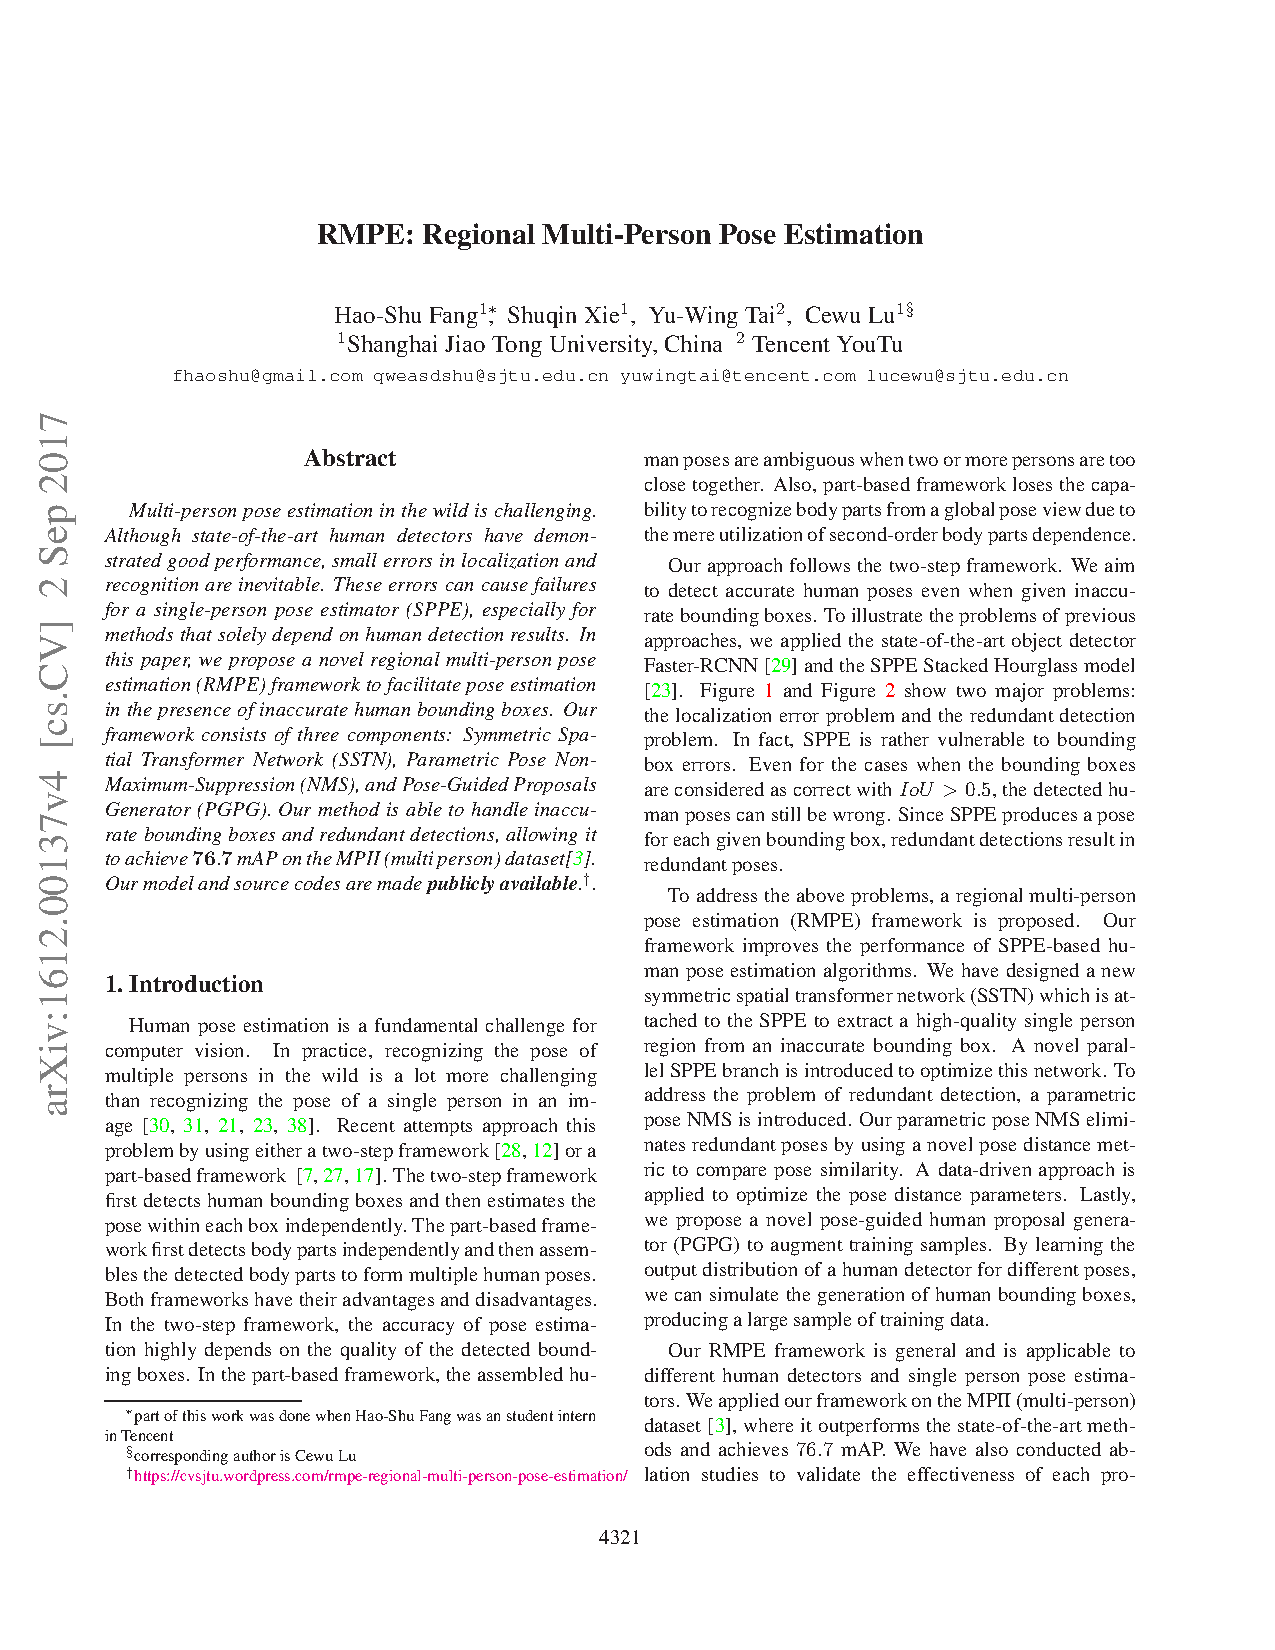
\includepdf[pages={1-}]{RMPE.pdf}
%  \input{data/appendix02}
% \end{appendix}
% \end{latex}
%
% \DescribeMacro{\title}
% 附录里主要是本科的外文资料以及翻译,在这种情况下,\cs{chapter} 的标题是固定的
% (即“外文资料的调研阅读报告或书面翻译”),所以用 \cs{title}\marg{标题} 开排版外
% 文资料以及翻译的标题。这个命令只能在附录环境下使用。
%
% \DescribeEnv{translationbib}
% 本环境用来描述外文资料中的参考文献,例子:
% \begin{latex}
% \begin{translationbib}
%   \item Donald E. Knuth. The \TeX book. Addison-Wesley, 1984. ISBN: 0-201-13448-9
%   \item Paul W. Abrahams, Karl Berry and Kathryn A. Hargreaves. \TeX\ for the
%     Impatient. Addison-Wesley, 1990. ISBN: 0-201-51375-7
%   \item David Salomon. The advanced \TeX book.  New York : Springer, 1995. ISBN:0-387-94556-3
% \end{translationbib}
% \end{latex}
%
% \subsubsection{简历}
% \DescribeEnv{resume}
% 开启个人简历章节,包括个人简历,发表文章,研究成果列表等。每个子项目请
% 用以下对应命令开启:\cs{xxxitem}\marg{subtitle}。
%
% \DescribeMacro{\resumeitem}
% 个人简历,用法:\cs{resumeitem}\{个人简历\}。简历内容部分没有格式要求,正常段
% 落排版。
%
% \DescribeMacro{\researchitem}
% 发表学术论文,用法:\cs{researchitem}\marg{类别},包括“学术论文”和“研究成果”两
% 个类别。分别用 \env{publications} 和 \env{achievements} 罗列。
%
% \DescribeEnv{publications}
% \DescribeMacro{\publicationskip}
% 用 \env{publications} 环境进行罗列发表的论文。按照学校要求,在学期间发表的学术
% 论文分以下三部分按顺序分别列出,每部分之间空 1 行,序号可连续排列:
% \begin{enumerate}
% \item 已经刊载的学术论文(本人是第一作者,或者导师为第一作者本人是第二作者)
% \item 尚未刊载,但已经接到正式录用函的学术论文(本人为第一作者,或者导师为第一
%   作者本人是第二作者)。
% \item 其他学术论文。可列出除上述两种情况以外的其他学术论文,但必须是已经刊载或
%   者收到正式录用函的论文。
% \end{enumerate}
%
% \env{publications} 环境支持每一部分分别编写,逻辑上更清楚,为了在环境之间支持
% 空行,需要利用 \cs{publicationskip} 控制。示例:
% \begin{latex}
%  \researchitem{发表的学术论文}
%
%  % 1. 已经刊载的学术论文
%  \begin{publications}
%    \item Yang Y, Ren T L, Zhang L T, et al. Miniature microphone with silicon-
%      based ferroelectric thin films. Integrated Ferroelectrics, 2003,
%      52:229-235. (SCI 收录, 检索号:758FZ.)
%    \item 杨轶, 张宁欣, 任天令, 等. 硅基铁电微声学器件中薄膜残余应力的研究. 中国机
%      械工程, 2005, 16(14):1289-1291. (EI 收录, 检索号:0534931 2907.)
%    \item 杨轶, 张宁欣, 任天令, 等. 集成铁电器件中的关键工艺研究. 仪器仪表学报,
%      2003, 24(S4):192-193. (EI 源刊.)
%  \end{publications}
%
%  % 2. 尚未刊载,但已经接到正式录用函的学术论文
%  \begin{publications}[before=\publicationskip,after=\publicationskip]
%    \item Yang Y, Ren T L, Zhu Y P, et al. PMUTs for handwriting recognition. In
%      press. (已被 Integrated Ferroelectrics 录用. SCI 源刊.)
%  \end{publications}
%
%  % 3. 其他学术论文。
%  \begin{publications}
%    \item Wu X M, Yang Y, Cai J, et al. Measurements of ferroelectric MEMS
%      microphones. Integrated Ferroelectrics, 2005, 69:417-429. (SCI 收录, 检索号
%      :896KM)
%    \item 贾泽, 杨轶, 陈兢, 等. 用于压电和电容微麦克风的体硅腐蚀相关研究. 压电与声
%      光, 2006, 28(1):117-119. (EI 收录, 检索号:06129773469)
%    \item 伍晓明, 杨轶, 张宁欣, 等. 基于MEMS技术的集成铁电硅微麦克风. 中国集成电路,
%      2003, 53:59-61.
%  \end{publications}
% \end{latex}
%
% \DescribeEnv{achievements}
% 研究成果用 \cs{researchitem}\{研究成果\} 开启,随后用 \env{achievements} 环
% 境罗列。
%
% 具体用法请参看示例文档 \file{data/resume.tex}。
%
% \subsection{书脊}
% \DescribeMacro{\shuji}
% 生成装订的书脊,为竖排格式,命令格式:\cs{shuji}\oarg{标题}\oarg{作者}。默认参
% 数为论文中文题目和中文作者。如果中文题目中没有英文字母,那么直接调用此命令即可。
% 否则,就要像例子里面那样做一些微调(参看模板自带的 \file{shuji.tex})。下面是一
% 个例子:
% \begin{latex}
% \documentclass[degree=master]{thuthesis}
%
% \begin{document}
% \thuset{
%   ctitle={论文中文题目},
%   cauthor={中文姓名}}
%
% \shuji % 使用默认标题和默认作者
%
% \shuji[使用默认作者的标题]
%
% \shuji[同时修改标题和作者的标题][尼瑞薛]
%
% % 如果标题中有英文,那可以参考如下方法进行微调:
% \shuji[北京工业大学 \raisebox{-5pt}{\LaTeX} 论文模板 \raisebox{-5pt}{v\version} 样例]
% \end{document}
% \end{latex}
%
% \subsection{自定义}
% \label{sec:othercmd}
%
% \subsubsection{数学环境}
% \label{sec:math}
% \thuthesis\ 定义了常用的数学环境:
%
% \begin{center}
% \begin{tabular}{*{7}{l}}\toprule
%   axiom & theorem & definition & proposition & lemma & conjecture &\\
%   公理 & 定理 & 定义 & 命题 & 引理 & 猜想 &\\\midrule
%   proof & corollary & example & exercise & assumption & remark & problem \\
%   证明 & 推论 & 例子& 练习 & 假设 & 注释 & 问题\\\bottomrule
% \end{tabular}
% \end{center}
%
% 比如:
% \begin{latex}
% \begin{definition}
%   道千乘之国,敬事而信,节用而爱人,使民以时。
% \end{definition}
% \end{latex}
% 产生(自动编号):
% \medskip
%
% \noindent\framebox[\linewidth][l]{{\heiti 定义~1.1~~~} % {道千乘之国,敬事而信,节用而爱人,使民以时。}}
%
% \smallskip
% 列举出来的数学环境毕竟是有限的,如果想用\emph{胡说}这样的数学环境,那么可以定义:
% \begin{latex}
% \newtheorem{nonsense}{胡说}[chapter]
% \end{latex}
%
% 然后这样使用:
% \begin{latex}
% \begin{nonsense}
%   契丹武士要来中原夺武林秘笈。—— 慕容博
% \end{nonsense}
% \end{latex}
% 产生(自动编号):
%
% \medskip
% \noindent\framebox[\linewidth][l]{{\heiti 胡说~1.1~~~} % {契丹武士要来中原夺武林秘笈。—— 慕容博}}
%
% \subsubsection{列表环境}
% \DescribeEnv{itemize}
% \DescribeEnv{enumerate}
% \DescribeEnv{description}
% 为了适合中文习惯,模板将这三个常用的列表环境用 \pkg{enumitem} 进行了纵向间距压
% 缩。一方面清除了多余空间,另一方面用户可以自己指定列表环境的样式(如标签符号,
% 缩进等)。细节请参看 \pkg{enumitem} 文档,此处不再赘述。
%
% \section{致谢}
% \label{sec:thanks}
% 感谢这些年来一直陪伴 \thuthesis\ 成长的新老同学!
%
% 欢迎各位到 \href{http://github.com/xueruini/thuthesis/}{\thuthesis\ Github 主页}贡献!
%
% \StopEventually{\PrintChanges\PrintIndex}
% \clearpage
%
% \section{实现细节}
%
% \subsection{基本信息}
%    \begin{macrocode}
%<cls>\NeedsTeXFormat{LaTeX2e}[1999/12/01]
%<cls>\ProvidesClass{thuthesis}
%<cls>[2019/04/16 5.5.1 Tsinghua University Thesis Template]
%    \end{macrocode}
%
% 检查编译引擎,要求使用 XeLaTeX。
%    \begin{macrocode}
\RequirePackage{ifxetex}
\ifxetex\else
  \ClassError{thuthesis}{You should use XeLaTeX}{}
  \end{document}
\fi
%    \end{macrocode}
%
% \subsection{定义选项}
% \label{sec:defoption}
% 定义论文类型以及是否涉密
% \changes{v2.4}{2006/04/14}{添加模板名称命令。}
% \changes{v2.5}{2006/05/19}{增加本科论文的提交选项 submit。}
% \changes{v2.5.1}{2006/05/24}{如果没有设置格式选项,报错。}
% \changes{v2.5.1}{2006/05/26}{submit 只能由本科用。}
% \changes{v2.5.3}{2006/06/03}{submit 选项的一个笔误。}
% \changes{v3.0}{2007/05/12}{删除 submit 选项。}
% \changes{v4.6}{2011/04/26}{增加 postdoctor 选项。}
% \changes{v4.8}{2014/11/25}{v4.7曾经想发布,但是一直没有做,于是就被跳过了,算是造一个段子吧。}
% \changes{v4.8.1}{2014/12/09}{按照 CTAN 的要求整理一下文件。}
%    \begin{macrocode}
%<*cls>
\hyphenation{Thu-Thesis}
\def\thuthesis{ThuThesis}
\def\version{5.5.1}
\RequirePackage{kvoptions}
\SetupKeyvalOptions{
  family=thu,
  prefix=thu@,
  setkeys=\kvsetkeys}
%    \end{macrocode}
%
% 用 \pkg{kvoptions} 的 \texttt{key=value} 方式来设置论文类型。
% \changes{v5.0.0}{2015/12/13}{使用 \pkg{kvoptions} 简化选项 type。}
% \changes{v5.4.2}{2017/12/18}{使用 degree 取代 type 选项。}
%    \begin{macrocode}
\DeclareStringOption[doctor]{degree}[doctor]
%    \end{macrocode}
%
% 论文是使用英文。
% \changes{v5.5.0}{2018/12/09}{增加选项使用英文模板。}
%    \begin{macrocode}
\DeclareStringOption[chinese]{language}[chinese]
%    \end{macrocode}
%
% 论文是否保密。
%    \begin{macrocode}
\DeclareBoolOption{secret}
%    \end{macrocode}
%
% 章目录中的英文是否用 Arial 字体(默认关闭),可以分别控制内容和页码部分。
%    \begin{macrocode}
\DeclareBoolOption{tocarialchapter}
\DeclareBoolOption{tocarialchapterentry}
\DeclareBoolOption{tocarialchapterpage}
%    \end{macrocode}
%
%
% \option{raggedbottom} 选项(默认打开)
% \changes{v4.8}{2013/03/05}{增加 noraggedbottom 选项。}
% \changes{v5.0.0}{2015/12/13}{norggedbottom 选项修改为 raggedbottom。}
%    \begin{macrocode}
\DeclareBoolOption[true]{raggedbottom}
%    \end{macrocode}
%
% 将选项传递给 \pkg{ctexbook}。
%    \begin{macrocode}
\DeclareDefaultOption{\PassOptionsToClass{\CurrentOption}{ctexbook}}
%    \end{macrocode}
%
% \changes{v2.5.1}{2006/05/24}{研究生院目录要 times,而教务处要 arial。}
% \changes{v2.5.1}{2006/05/26}{本科 openright,研究生 openany。}
% \changes{v3.1}{2007/10/09}{本科的目录又不要 arial 字体了。}
% \changes{v4.8}{2013/05/29}{添加 nocap 选项,恢复默认标题样式,模板会进一步定制。}
% 解析用户传递过来的选项,并加载 \pkg{ctexbook}。
%    \begin{macrocode}
\ProcessKeyvalOptions*
\newcommand\thu@validate@key[1]{%
  \@ifundefined{thu@\csname thu@#1\endcsname true}{%
    \ClassError{thuthesis}{Invalid value '\csname thu@#1\endcsname'}{}%
  }{%
    \csname thu@\csname thu@#1\endcsname true\endcsname
  }%
}
\newif\ifthu@bachelor
\newif\ifthu@master
\newif\ifthu@doctor
\newif\ifthu@postdoctor
\thu@validate@key{degree}
\newif\ifthu@chinese
\newif\ifthu@english
\thu@validate@key{language}
%    \end{macrocode}
%
% \changes{v5.3.1}{2016/03/20}{使用 \CTeX\ 默认中文字体配置,支持不同引擎。}
% 使用 \pkg{ctexbook} 类,优于调用 \pkg{ctex} 宏包。
%    \begin{macrocode}
\PassOptionsToPackage{quiet}{xeCJK}
\LoadClass[a4paper,openany,UTF8,zihao=-4,scheme=plain]{ctexbook}
%    \end{macrocode}
%
%
% \subsection{装载宏包}
% \label{sec:loadpackage}
%
% 引用的宏包和相应的定义。
%    \begin{macrocode}
\RequirePackage{etoolbox}
\RequirePackage{xparse}
%    \end{macrocode}
%
% \AmSTeX\ 宏包,用来排出更加漂亮的公式。
% \changes{v4.8}{2013/03/02}{no need to load amssymb since we use txfonts.}
%    \begin{macrocode}
\RequirePackage{amsmath}
%    \end{macrocode}
%
% 使用 \pkg{unicode-math} 处理数学字体。
% \changes{v3.1}{2007/06/16}{replace \pkg{mathptmx} with \pkg{txfonts}.}
% \changes{v5.2.1}{2016/01/14}{使用 \pkg{newtx} 替换 \pkg{txfonts}。}
% \changes{v5.2.2}{2016/02/01}{不希望 \pkg{newtx} 修改 \cs{@makefnmark}。 }
% \changes{v5.5.0}{2018/07/07}{使用 \pkg{unicode-math} 处理数学字体。}
%    \begin{macrocode}
\RequirePackage{unicode-math}
%    \end{macrocode}
%
% 图形支持宏包。
%    \begin{macrocode}
\RequirePackage{graphicx}
%    \end{macrocode}
%
% 并排图形。\pkg{subfigure}、\pkg{subfig} 已经不再推荐,用新的 \pkg{subcaption}。
% 浮动图形和表格标题样式。\pkg{caption2} 已经不推荐使用,采用新的 \pkg{caption}。
%    \begin{macrocode}
\RequirePackage[labelformat=simple]{subcaption}
%    \end{macrocode}
%
% \pkg{pdfpages} 宏包便于我们插入扫描后的授权页和声明页 PDF 文档。
%    \begin{macrocode}
\RequirePackage{pdfpages}
\includepdfset{fitpaper=true}
%    \end{macrocode}
%
% 更好的列表环境。
% \changes{v2.6.2}{2006/06/18}{去掉 \pkg{paralist} 的 \option{newitem} 和
% \option{newenum} 选项,因为默认是打开的。}
% \changes{v2.6.4}{2006/10/23}{增加 \option{neverdecrease} 选项。}
% \changes{v5.0.0}{2012/12/13}{删除 \pkg{paralist} 选项。}
% \changes{v5.2.2}{2016/01/31}{利用 \pkg{environ} 的 \cs{Collect@Body}。}
%    \begin{macrocode}
\RequirePackage[shortlabels]{enumitem}
\RequirePackage{environ}
%    \end{macrocode}
%
% 禁止 \LaTeX 自动调整多余的页面底部空白,并保持脚注仍然在底部。
% 脚注按页编号。
%    \begin{macrocode}
\ifthu@raggedbottom
  \RequirePackage[bottom,perpage,hang]{footmisc}
  \raggedbottom
\else
  \RequirePackage[perpage,hang]{footmisc}
\fi
%    \end{macrocode}
%
% 利用 \pkg{CJKfntef} 实现汉字的下划线和盒子内两段对齐,并可以避免
% \cs{makebox}\oarg{width}\oarg{s} 可能产生的 underful boxes。
%    \begin{macrocode}
\RequirePackage{CJKfntef}
%    \end{macrocode}
%
% \changes{v4.8}{2013/05/28}{在 CJK 模式下用 \pkg{CJKspace} 保留中英文间空格。}
% \changes{v5.0.0}{2015/04/17}{固定字体设置,同时改善与 \pkg{ctex} 兼容性。}
% \changes{v5.2.1}{2016/01/14}{使用 \pkg{newtx} 字体。}
% \changes{v5.3.1}{2016/03/20}{\pkg{ctex} 默认加载 \pkg{CJKspace}。}
% \changes{v5.3.1}{2016/03/20}{几乎没人主动安装 Arial 字体。}
%
% 定理类环境宏包,其中 \pkg{amsmath} 选项用来兼容 \AmSTeX\ 的宏包
%    \begin{macrocode}
\RequirePackage[amsmath,thmmarks,hyperref]{ntheorem}
%    \end{macrocode}
%
% 表格控制
% \changes{v2.6}{2006/06/09}{增加 \pkg{longtable}。}
%    \begin{macrocode}
\RequirePackage{array}
\RequirePackage{longtable}
%    \end{macrocode}
%
% 使用三线表:\cs{toprule},\cs{midrule},\cs{bottomrule}。
%    \begin{macrocode}
\RequirePackage{booktabs}
%    \end{macrocode}
%
% 参考文献引用宏包。
%    \begin{macrocode}
\RequirePackage[sort&compress]{natbib}
%    \end{macrocode}
%
% 删除默认模板(\file{book.cls})在章之间引入的垂直间隔。要放在 \pkg{hyperref}
% 之前。
%    \begin{macrocode}
%    \end{macrocode}
% 生成有书签的 pdf 及其开关,请结合 gbk2uni 避免书签乱码。
% \changes{v2.6}{2006/06/09}{去除 hyperref 选项,等待全局传递。}
% \changes{v5.2.2}{2016/01/25}{目录中标题和页码都是链接。}
%    \begin{macrocode}
\RequirePackage{hyperref}
\hypersetup{
  linktoc            = all,
  bookmarksnumbered  = true,
  bookmarksopen      = true,
  bookmarksopenlevel = 1,
  breaklinks         = true,
  plainpages         = false,
  hidelinks,
}
\pdfstringdefDisableCommands{
  \let\\\@empty
  \let\hspace\@gobble
}
%    \end{macrocode}
%
% 设置 url 样式,与上下文一致
%    \begin{macrocode}
\urlstyle{same}
%    \end{macrocode}
%
% 使用 \pkg{xurl} 的方法,增加 URL 可断行的位置。
%    \begin{macrocode}
\def\UrlBreaks{%
  \do\/%
  \do\a\do\b\do\c\do\d\do\e\do\f\do\g\do\h\do\i\do\j\do\k\do\l%
     \do\m\do\n\do\o\do\p\do\q\do\r\do\s\do\t\do\u\do\v\do\w\do\x\do\y\do\z%
  \do\A\do\B\do\C\do\D\do\E\do\F\do\G\do\H\do\I\do\J\do\K\do\L%
     \do\M\do\N\do\O\do\P\do\Q\do\R\do\S\do\T\do\U\do\V\do\W\do\X\do\Y\do\Z%
  \do0\do1\do2\do3\do4\do5\do6\do7\do8\do9\do=\do/\do.\do:%
  \do\*\do\-\do\~\do\'\do\"\do\-}
\Urlmuskip=0mu plus 0.1mu
%    \end{macrocode}
%
%
% \subsection{页面设置}
% \label{sec:layout}
% 本来这部分应该是最容易设置的,但根据格式规定出来的结果跟学校的 WORD 样例相差很
% 大,所以只能微调。
% \changes{v2.4}{2006/04/14}{把页面尺寸写入 dvi,避免有的用户通
%   过 dvips 不指定页面类型而得到古怪的结果。}
% \changes{v4.5.2}{2010/09/19}{研究生页面边距由 3.2cm 改为 3cm。}
% \changes{v4.7}{2012/05/29}{修改本科生页脚间距与样例基本一致。}
% \changes{v5.0.0}{2015/03/10}{不再将页面尺寸写入 dvi,因为已不支持 dvips,
% 而该方案会使得在使用 tikzexternalize 时外部 PDF 图片 BBox 不对。}
% \changes{v5.0.0}{2015/12/14}{用 \pkg{geometry} 简化设置。}
%    \begin{macrocode}
\RequirePackage{geometry}
\geometry{
  a4paper, % 210 * 297mm
  hcentering,
  ignoreall,
  nomarginpar}
\ifthu@bachelor
  \geometry{
    left=32mm,
    headheight=5mm,
    headsep=5mm,
    textheight=227mm,
    bottom=32mm,
    footskip=12mm}
\else
  \geometry{
    left=30mm,
    headheight=5mm,
    headsep=5mm,
    textheight=237mm,
    bottom=29mm,
    footskip=6mm}
\fi
%    \end{macrocode}
%
% 利用 \pkg{fancyhdr} 设置页眉页脚。
%    \begin{macrocode}
\RequirePackage{fancyhdr}
%    \end{macrocode}
%
% 利用 \pkg{notoccite} 避免目录中引用编号混乱。
% \changes{v5.4.4}{2018/04/13}{让目录中的引用不影响正文中引用序号。}
%    \begin{macrocode}
\RequirePackage{notoccite}
%    \end{macrocode}
%
% \subsection{主文档格式}
% \label{sec:mainbody}
%
% \subsubsection{Three matters}
% \begin{macro}{\cleardoublepage}
% 对于 \textsl{openright} 选项,必须保证章首页右开,且如果前章末页无内容须
% 清空其页眉页脚。
%    \begin{macrocode}
\let\thu@cleardoublepage\cleardoublepage
\newcommand{\thu@clearemptydoublepage}{%
  \clearpage{\pagestyle{thu@empty}\thu@cleardoublepage}}
\let\cleardoublepage\thu@clearemptydoublepage
%    \end{macrocode}
% \end{macro}
%
% \begin{macro}{\frontmatter}
% \begin{macro}{\mainmatter}
% \begin{macro}{\backmatter}
% 我们的单面和双面模式与常规的不太一样。
% \changes{v2.5.1}{2006/05/23}{本科正文之后页码即用罗马数字,研究生不变。}
% \changes{v2.5.3}{2006/06/03}{第一章永远右开。}
% \changes{v4.4}{2008/05/30}{本科正文后的页码延续前面的阿拉伯数字,不再用罗马数
% 字。}
% \changes{v4.4}{2008/05/30}{本科取消了所有页眉。}
%    \begin{macrocode}
\renewcommand\frontmatter{%
  \if@openright\cleardoublepage\else\clearpage\fi
  \@mainmatterfalse
  \pagenumbering{Alph}
  \pagestyle{thu@empty}}
\renewcommand\mainmatter{%
  \if@openright\cleardoublepage\else\clearpage\fi
  \@mainmattertrue
  \pagenumbering{arabic}
  \ifthu@bachelor\pagestyle{thu@plain}\else\pagestyle{thu@headings}\fi}
\renewcommand\backmatter{%
  \if@openright\cleardoublepage\else\clearpage\fi
  \@mainmattertrue}
%    \end{macrocode}
% \end{macro}
% \end{macro}
% \end{macro}
%
% \subsubsection{字体}
% \label{sec:font}
% 使用 \pkg{fontspec} 配置字体。
%    \begin{macrocode}
\newcommand\thu@fontset{\csname g__ctex_fontset_tl\endcsname}
\ifthenelse{\equal{\thu@fontset}{fandol}}{
  \setmainfont[
    Extension      = .otf,
    UprightFont    = *-regular,
    BoldFont       = *-bold,
    ItalicFont     = *-italic,
    BoldItalicFont = *-bolditalic,
  ]{texgyretermes}
  \setsansfont[
    Extension      = .otf,
    UprightFont    = *-regular,
    BoldFont       = *-bold,
    ItalicFont     = *-italic,
    BoldItalicFont = *-bolditalic,
  ]{texgyreheros}
  \setmonofont[
    Extension      = .otf,
    UprightFont    = *-regular,
    BoldFont       = *-bold,
    ItalicFont     = *-italic,
    BoldItalicFont = *-bolditalic,
    Scale          = MatchLowercase,
  ]{texgyrecursor}
}{
  \setmainfont{Times New Roman}
  \setsansfont{Arial}
  \ifthenelse{\equal{\thu@fontset}{mac}}{
    \setmonofont[Scale=MatchLowercase]{Menlo}
  }{
    \setmonofont[Scale=MatchLowercase]{Courier New}
  }
}
%    \end{macrocode}
%
% 使用 \pkg{unicode-math} 配置数学字体
% \changes{v5.5.2}{2019/04/21}{使用 XITS 数学字体。}
%    \begin{macrocode}
\unimathsetup{
  math-style = ISO,
  bold-style = ISO,
  nabla      = upright,
  partial    = upright,
}
\IfFontExistsTF{XITSMath-Regular.otf}{
  \setmathfont[
    Extension    = .otf,
    BoldFont     = XITSMath-Bold,
    StylisticSet = 8,
  ]{XITSMath-Regular}
  \setmathfont[range={cal,bfcal},StylisticSet=1]{XITSMath-Regular.otf}
}{
  \setmathfont[
    Extension    = .otf,
    BoldFont     = *bold,
    StylisticSet = 8,
  ]{xits-math}
  \setmathfont[range={cal,bfcal},StylisticSet=1]{xits-math.otf}
}
%    \end{macrocode}
%
% 在使用 Windows Vista 或之后版本的系统时,\pkg{ctex} 宏包会默认使用微软雅黑字体,
% 这可能会导致审查不合格。下面设置适合印刷的黑体,同时保持跨平台兼容性。
% \changes{v5.5.0}{2019/01/06}{Windows 的中文字体开启伪粗。}
%    \begin{macrocode}
\ifthenelse{\equal{\thu@fontset}{windows}}{
  \xeCJKsetup{EmboldenFactor=2}
  \IfFileExists{C:/bootfont.bin}{
    \setCJKmainfont[AutoFakeBold,ItalicFont=KaiTi_GB2312]{SimSun}
    \setCJKfamilyfont{zhkai}[AutoFakeBold]{KaiTi_GB2312}
  }{
    \setCJKmainfont[AutoFakeBold,ItalicFont=KaiTi]{SimSun}
    \setCJKfamilyfont{zhkai}[AutoFakeBold]{KaiTi}
  }
  \setCJKsansfont[AutoFakeBold]{SimHei}
  \setCJKfamilyfont{zhsong}[AutoFakeBold]{SimSun}
  \setCJKfamilyfont{zhhei}[AutoFakeBold]{SimHei}
}{}
%    \end{macrocode}
%
% 类似地,\pkg{ctex} 2.4.14 开始在 macOS 下自动调用苹方黑体,所以必进行调整。
%    \begin{macrocode}
\ifthenelse{\equal{\thu@fontset}{mac}}{
  \setCJKmainfont[
         UprightFont = * Light,
            BoldFont = * Bold,
          ItalicFont = Kaiti SC,
      BoldItalicFont = Kaiti SC Bold,
    ]{Songti SC}
  \setCJKsansfont[BoldFont=* Medium]{Heiti SC}
  \setCJKfamilyfont{zhsong}[
         UprightFont = * Light,
            BoldFont = * Bold,
    ]{Songti SC}
  \setCJKfamilyfont{zhhei}[BoldFont=* Medium]{Heiti SC}
  \setCJKfamilyfont{zhkai}[BoldFont=* Bold]{Kaiti SC}
  \xeCJKsetwidth{‘’“”}{1em}
}{}
%    \end{macrocode}
%
% \begin{macro}{\normalsize}
% 正文小四号 (12bp) 字,行距为固定值 20 bp。
% \changes{v5.4.5}{2018/05/17}{调整公式和正文间距。}
%    \begin{macrocode}
\renewcommand\normalsize{%
  \@setfontsize\normalsize{12bp}{20bp}%
  \abovedisplayskip=12bp \@plus 2bp \@minus 2bp
  \abovedisplayshortskip=12bp \@plus 2bp \@minus 2bp
  \belowdisplayskip=\abovedisplayskip
  \belowdisplayshortskip=\abovedisplayshortskip}
%    \end{macrocode}
% \end{macro}
%
% WORD 中的字号对应该关系如下(1bp = 72.27/72 pt):
% \begin{center}
% \begin{tabular}{llll}
% \toprule
% 初号 & 42bp & 14.82mm & 42.1575pt \\
% 小初 & 36bp & 12.70mm & 36.135 pt \\
% 一号 & 26bp & 9.17mm & 26.0975pt \\
% 小一 & 24bp & 8.47mm & 24.09pt \\
% 二号 & 22bp & 7.76mm & 22.0825pt \\
% 小二 & 18bp & 6.35mm & 18.0675pt \\
% 三号 & 16bp & 5.64mm & 16.06pt \\
% 小三 & 15bp & 5.29mm & 15.05625pt \\
% 四号 & 14bp & 4.94mm & 14.0525pt \\
% 小四 & 12bp & 4.23mm & 12.045pt \\
% 五号 & 10.5bp & 3.70mm & 10.59375pt \\
% 小五 & 9bp & 3.18mm & 9.03375pt \\
% 六号 & 7.5bp & 2.56mm & \\
% 小六 & 6.5bp & 2.29mm & \\
% 七号 & 5.5bp & 1.94mm & \\
% 八号 & 5bp & 1.76mm & \\\bottomrule
% \end{tabular}
% \end{center}
%
% \begin{macro}{\thu@def@fontsize}
% \changes{v2.6.2}{2006/06/18}{引入此命令重新定义字号。}
% 根据习惯定义字号。用法:
%
% \cs{thu@def@fontsize}\marg{字号名称}\marg{磅数}
%
% 避免了字号选择和行距的紧耦合。所有字号定义时为单倍行距,并提供选项指定行距倍数。
% \changes{v5.2.3}{2016/02/13}{改写字体定义命令。}
%    \begin{macrocode}
\def\thu@def@fontsize#1#2{%
  \expandafter\newcommand\csname #1\endcsname[1][1.3]{%
    \fontsize{#2}{##1\dimexpr #2}\selectfont}}
%    \end{macrocode}
% \end{macro}
%
% \begin{macro}{\chuhao}
% \begin{macro}{\xiaochu}
% \begin{macro}{\yihao}
% \begin{macro}{\xiaoyi}
% \begin{macro}{\erhao}
% \begin{macro}{\xiaoer}
% \begin{macro}{\sanhao}
% \begin{macro}{\xiaosan}
% \begin{macro}{\sihao}
% \begin{macro}{\banxiaosi}
% \begin{macro}{\xiaosi}
% \begin{macro}{\dawu}
% \begin{macro}{\wuhao}
% \begin{macro}{\xiaowu}
% \begin{macro}{\liuhao}
% \begin{macro}{\xiaoliu}
% \begin{macro}{\qihao}
% \begin{macro}{\bahao}
% 一组字号定义。TODO:用 \cs{zihao} 替代。
%    \begin{macrocode}
\thu@def@fontsize{chuhao}{42bp}
\thu@def@fontsize{xiaochu}{36bp}
\thu@def@fontsize{yihao}{26bp}
\thu@def@fontsize{xiaoyi}{24bp}
\thu@def@fontsize{erhao}{22bp}
\thu@def@fontsize{xiaoer}{18bp}
\thu@def@fontsize{sanhao}{16bp}
\thu@def@fontsize{xiaosan}{15bp}
\thu@def@fontsize{sihao}{14bp}
\thu@def@fontsize{banxiaosi}{13bp}
\thu@def@fontsize{xiaosi}{12bp}
\thu@def@fontsize{dawu}{11bp}
\thu@def@fontsize{wuhao}{10.5bp}
\thu@def@fontsize{xiaowu}{9bp}
\thu@def@fontsize{liuhao}{7.5bp}
\thu@def@fontsize{xiaoliu}{6.5bp}
\thu@def@fontsize{qihao}{5.5bp}
\thu@def@fontsize{bahao}{5bp}
%    \end{macrocode}
% \end{macro}
% \end{macro}
% \end{macro}
% \end{macro}
% \end{macro}
% \end{macro}
% \end{macro}
% \end{macro}
% \end{macro}
% \end{macro}
% \end{macro}
% \end{macro}
% \end{macro}
% \end{macro}
% \end{macro}
% \end{macro}
% \end{macro}
% \end{macro}
%
%
% \subsubsection{语言设置}
%
% \newcommand\unicodechar[1]{U+#1(\symbol{"#1})}
% 由于 Unicode 的一些标点符号是中西文混用的:
% \unicodechar{00B7}、
% \unicodechar{2013}、
% \unicodechar{2014}、
% \unicodechar{2018}、
% \unicodechar{2019}、
% \unicodechar{201C}、
% \unicodechar{201D}、
% \unicodechar{2025}、
% \unicodechar{2026}、
% \unicodechar{2E3A},
% 所以要根据语言设置正确的字体。
% \footnote{\url{https://github.com/CTeX-org/ctex-kit/issues/389}}
% 所以要根据语言设置正确的字体。
%    \begin{macrocode}
\newcommand\thu@setchinese{%
  \xeCJKResetPunctClass
}
\newcommand\thu@setenglish{%
  \xeCJKDeclareCharClass{HalfLeft}{"2018, "201C}%
  \xeCJKDeclareCharClass{HalfRight}{
    "00B7, "2019, "201D, "2013, "2014, "2025, "2026, "2E3A,
  }%
}
\newcommand\thu@setdefaultlanguage{%
  \ifthu@chinese
    \thu@setchinese
  \else
    \thu@setenglish
  \fi
}
%    \end{macrocode}
%
% 中英文翻译:
%    \begin{macrocode}
\ifthu@chinese
  \ctexset{
    chapter/name   = {第,章},
    appendixname   = 附录,
    contentsname   = {目\hspace{\ccwd}录},
    listfigurename = 插图索引,
    listtablename  = 表格索引,
    figurename     = 图,
    tablename      = 表,
    bibname        = 参考文献,
    indexname      = 索引,
  }
  \newcommand\thu@denotation@name{主要符号对照表}
  \newcommand\listequationname{公式索引}
  \newcommand\equationname{公式}
  \newcommand\thu@assumption@name{假设}
  \newcommand\thu@definition@name{定义}
  \newcommand\thu@proposition@name{命题}
  \newcommand\thu@lemma@name{引理}
  \newcommand\thu@theorem@name{定理}
  \newcommand\thu@axiom@name{公理}
  \newcommand\thu@corollary@name{推论}
  \newcommand\thu@exercise@name{练习}
  \newcommand\thu@example@name{例}
  \newcommand\thu@remark@name{注释}
  \newcommand\thu@problem@name{问题}
  \newcommand\thu@conjecture@name{猜想}
  \newcommand\thu@proof@name{证明}
  \newcommand\thu@theorem@separator{:}
  \newcommand\thu@ack@name{致\hspace{\ccwd}谢}
  \ifthu@bachelor
    \newcommand\thu@resume@title{在学期间参加课题的研究成果}
  \else
    \ifthu@postdoctor
      \newcommand\thu@resume@title{个人简历、发表的学术论文与科研成果}
    \else
      \newcommand\thu@resume@title{个人简历、在学期间发表的学术论文与研究成果}
    \fi
  \fi
\else
  \newcommand\thu@denotation@name{Nomenclature}
  \newcommand\listequationname{List of Equations}
  \newcommand\equationname{Equation}
  \newcommand\thu@assumption@name{Assumption}
  \newcommand\thu@definition@name{Definition}
  \newcommand\thu@proposition@name{Proposition}
  \newcommand\thu@lemma@name{Lemma}
  \newcommand\thu@theorem@name{Theorem}
  \newcommand\thu@axiom@name{Axiom}
  \newcommand\thu@corollary@name{Corollary}
  \newcommand\thu@exercise@name{Exercise}
  \newcommand\thu@example@name{Example}
  \newcommand\thu@remark@name{Remark}
  \newcommand\thu@problem@name{Problem}
  \newcommand\thu@conjecture@name{Conjecture}
  \newcommand\thu@proof@name{proof}
  \newcommand\thu@theorem@separator{: }
  \newcommand\thu@ack@name{Acknowledgments}
  \ifthu@bachelor
    \newcommand\thu@resume@title{Research Achievements}
  \else
    \ifthu@postdoctor
      \newcommand\thu@resume@title{%
        Resume, Publications and Research Achievements%
      }
    \else
      \newcommand\thu@resume@title{%
        Resume, Publications and Research Achievements%
      }
    \fi
  \fi
\fi
%    \end{macrocode}
%
%
% \subsubsection{页眉页脚}
% \label{sec:headerfooter}
%
% 定义页眉和页脚。
% \begin{macro}{\ps@thu@empty}
% \begin{macro}{\ps@thu@plain}
% \begin{macro}{\ps@thu@headings}
% \changes{v2.0}{2005/12/18}{以前的太乱了,重新整理过清晰多了。}
% \changes{v2.1}{2006/03/01}{彻底放弃 fancyhdr,定义自己的样式。}
% \changes{v2.5}{2006/05/13}{本科的奇偶页眉不同。}
% \changes{v2.5}{2006/05/20}{增加 empty 页面样式。}
% \changes{v4.7}{2012/05/29}{本科页码用小五号字。}
% \changes{v5.0.0}{2015/12/20}{利用 \pkg{fancyhdr} 设置页眉页脚。}
% 定义三种页眉页脚格式:
% \begin{itemize}
% \item \texttt{thu@empty}:页眉页脚都没有
% \item \texttt{thu@plain}:只显示页脚的页码。\cs{chapter} 自动调用
% \cs{thispagestyle\{thu@plain\}}。
% \item \texttt{thu@headings}:页眉页脚同时显示
% \end{itemize}
%    \begin{macrocode}
\fancypagestyle{thu@empty}{%
  \fancyhf{}
  \renewcommand{\headrulewidth}{0pt}
  \renewcommand{\footrulewidth}{0pt}}
\fancypagestyle{thu@plain}{%
  \fancyhead{}
  \fancyhead[C]{\lishu \sanhao 北京工业大学毕业设计(论文)}
  \fancyfoot{}
  \fancyfoot[C]{\wuhao\thepage}
  \renewcommand{\headrulewidth}{1pt}
  \renewcommand{\footrulewidth}{0pt}}
\fancypagestyle{thu@headings}{%
  \fancyhead{}
  \fancyhead[C]{\wuhao\normalfont\leftmark}
  \fancyfoot{}
  \fancyfoot[C]{\wuhao\thepage}
  \renewcommand{\headrulewidth}{0.4pt}
  \renewcommand{\footrulewidth}{0pt}}
%    \end{macrocode}
% \end{macro}
% \end{macro}
% \end{macro}
%
%
% \subsubsection{段落}
% \label{sec:paragraph}
%
% 全文首行缩进 2 字符,标点符号用全角
%    \begin{macrocode}
\ctexset{%
  punct=quanjiao,
  space=auto,
  autoindent=true}
%    \end{macrocode}
%
% 利用 \pkg{enumitem} 命令调整默认列表环境间的距离,以符合中文习惯。
% \changes{v2.5.2}{2006/06/01}{更改默认列表距离。}
%    \begin{macrocode}
\setlist{nosep}
%    \end{macrocode}
%
%
% \subsubsection{脚注}
% \label{sec:footnote}
% 脚注符合中文习惯,数字带圈。
% \changes{v2.1}{2006/03/01}{让脚注它悬挂起来,而且中文中用上标,脚注中用正体。}
% \changes{v2.5}{2006/05/13}{修正 minipage 中的脚注。}
% \begin{macro}{\thu@textcircled}
% \changes{v2.5.1}{2006/05/21}{脚注编号使用 \cs{textcircled} 命令,每页允许至多 99 个。}
% \changes{v5.2.2}{2016/02/01}{脚注编号每页允许至多 9 个。}
% \changes{v5.5.0}{2018/12/10}{去掉 \option{pifootnote} 选项。}
% \changes{v5.5.1}{2019/04/16}{修复 minipage 中 footnote 编号问题。}
% 生成带圈的脚注数字,最多处理到 10。
%    \begin{macrocode}
\ifthenelse{\equal{\thu@fontset}{mac}}{
  \newfontfamily\thu@circlefont{Songti SC Light}
}{
  \ifthenelse{\equal{\thu@fontset}{windows}}{
    \newfontfamily\thu@circlefont{SimSun}
  }{
    \IfFontExistsTF{XITS-Regular.otf}{
      \newfontfamily\thu@circlefont{XITS-Regular.otf}
    }{
      \newfontfamily\thu@circlefont{xits-regular.otf}
    }
  }
}
\def\thu@textcircled#1{%
  \ifnum\value{#1} >9%
    \ClassError{thuthesis}%
      {Too many footnotes in this page.}{Keep footnote less than 10.}%
  \fi
  {\thu@circlefont\symbol{\the\numexpr\value{#1}+"245F\relax}}%
}
\renewcommand{\thefootnote}{\thu@textcircled{footnote}}
\renewcommand{\thempfootnote}{\thu@textcircled{mpfootnote}}
%    \end{macrocode}
% \end{macro}
%
% 定义脚注分割线,字号(宋体小五),以及悬挂缩进(1.5字符)。
%    \begin{macrocode}
\def\footnoterule{\vskip-3\p@\hrule\@width0.3\textwidth\@height0.4\p@\vskip2.6\p@}
\let\thu@footnotesize\footnotesize
\renewcommand\footnotesize{\thu@footnotesize\xiaowu[1.5]}
\footnotemargin1.5em\relax
%    \end{macrocode}
%
% \cs{@makefnmark} 默认是上标样式,而在脚注部分要求为正文大小。利用\cs{patchcmd}
% 动态调整 \cs{@makefnmark} 的定义。
% \changes{v2.6}{2006/06/09}{脚注改成 1.5 倍行距,漂亮。}
% \changes{v5.2.2}{2016/02/01}{基于 \pkg{footmisc} 来设置不同位置 footnote
% marker 样式。}
%    \begin{macrocode}
\let\thu@makefnmark\@makefnmark
\def\thu@@makefnmark{\hbox{{\normalfont\@thefnmark}}}
\pretocmd{\@makefntext}{\let\@makefnmark\thu@@makefnmark}{}{}
\apptocmd{\@makefntext}{\let\@makefnmark\thu@makefnmark}{}{}
%    \end{macrocode}
%
%
% \subsubsection{数学相关}
% \label{sec:equation}
% \begin{macro}{\ldots}
% 省略号一律居中,所以 \cs{ldots} 不再居于底部。
%    \begin{macrocode}
\ifthu@chinese
  \def\mathellipsis{\cdots}
\fi
%    \end{macrocode}
% \end{macro}
%
% \begin{macro}{\le}
% \begin{macro}{\ge}
% \begin{macro}{\leq}
% \begin{macro}{\geq}
% 小于等于号要使用倾斜的形式。
%    \begin{macrocode}
\protected\def\le{\leqslant}
\protected\def\ge{\geqslant}
\AtBeginDocument{%
  \renewcommand\leq{\leqslant}%
  \renewcommand\geq{\geqslant}%
}
%    \end{macrocode}
% \end{macro}
% \end{macro}
% \end{macro}
% \end{macro}
%
% \begin{macro}{\int}
% 积分号 \cs{int} 使用正体,并且上下限默认置于积分号上下两侧。
%    \begin{macrocode}
\removenolimits{%
  \int\iint\iiint\iiiint\oint\oiint\oiiint
  \intclockwise\varointclockwise\ointctrclockwise\sumint
  \intbar\intBar\fint\cirfnint\awint\rppolint
  \scpolint\npolint\pointint\sqint\intlarhk\intx
  \intcap\intcup\upint\lowint
}
%    \end{macrocode}
% \end{macro}
%
% \begin{macro}{\Re}
% \begin{macro}{\Im}
% 实部、虚部操作符使用罗马体 $\mathrm{Re}$、$\mathrm{Im}$ 而不是 fraktur 体
% $\Re$、$\Im$。
%    \begin{macrocode}
\AtBeginDocument{%
  \renewcommand{\Re}{\operatorname{Re}}%
  \renewcommand{\Im}{\operatorname{Im}}%
}
%    \end{macrocode}
% \end{macro}
% \end{macro}
%
% \begin{macro}{\nabla}
% \cs{nabla} 使用粗正体。
%    \begin{macrocode}
\AtBeginDocument{%
  \renewcommand\nabla{\mbfnabla}%
}
%    \end{macrocode}
% \end{macro}
%
% \begin{macro}{\bm}
% \begin{macro}{\boldsymbol}
% 兼容旧的粗体命令:\pkg{bm} 的 \cs{bm} 和 \pkg{amsmath} 的 \cs{boldsymbol}。
%    \begin{macrocode}
\newcommand\bm{\symbf}
\renewcommand\boldsymbol{\symbf}
%    \end{macrocode}
% \end{macro}
% \end{macro}
%
% \begin{macro}{\square}
% 兼容 \pkg{amssymb} 中的命令。
%    \begin{macrocode}
\newcommand\square{\mdlgwhtsquare}
%    \end{macrocode}
% \end{macro}
%
% 允许太长的公式断行、分页等。
%    \begin{macrocode}
\allowdisplaybreaks[4]
\renewcommand\theequation{\ifnum \c@chapter>\z@ \thechapter-\fi\@arabic\c@equation}
%    \end{macrocode}
%
% 公式距前后文的距离由 4 个参数控制,参见 \cs{normalsize} 的定义。
%
% \changes{v2.5.1}{2006/05/24}{本科公式编号前添加\textbf{公式}二字。需要修 \pkg{amsmath} 极其深的一个命令。}
% \changes{v2.5.1}{2006/05/24}{教务处居然要本科论文公式全文编号!}
% \changes{v2.5.2}{2006/05/29}{上一个版本忘了把研究生的公式编号排除。}
% \changes{v3.0}{2007/05/12}{本科公式又要取消全文统一编号了。}
% 本科的公式编号要求很诡异,不得不修改 \pkg{amsmath} 中很深的一个命令 \cs{tagform@}。
% \changes{v2.6.2}{2006/06/19}{根据不同论文格式显示不同公式编号,并自动加入索引。}
% \changes{v4.2}{2008/01/23}{\cs{eqref} 加括号。}
% 同时为了让 \pkg{amsmath} 的 \cs{tag*} 命令得到正确的格式,我们必须修改这些代
% 码。\cs{make@df@tag} 是定义 \cs{tag*} 和 \cs{tag} 内部命令的。
% \cs{make@df@tag@@} 处理 \cs{tag*},我们就改它!
% \begin{latex}
% \def\make@df@tag{\@ifstar\make@df@tag@@\make@df@tag@@@}
% \def\make@df@tag@@#1{%
%   \gdef\df@tag{\maketag@@@{#1}\def\@currentlabel{#1}}}
% \end{latex}
% \changes{v4.4}{2008/05/30}{本科论文终于去掉了\textbf{公式}二字。}
% \changes{v4.4.4}{2008/06/12}{修复了一个从 v4.3 升级到 v4.4 过程中的丢失公式索引的 bug,原修改代码保留备忘。}
% \changes{v5.2.3}{2016/02/13}{安全注释本科公式部分。}
%    \begin{macrocode}
\def\make@df@tag{\@ifstar\thu@make@df@tag@@\make@df@tag@@@}
\def\thu@make@df@tag@@#1{\gdef\df@tag{\thu@maketag{#1}\def\@currentlabel{#1}}}
\iffalse
\ifthu@bachelor
  \def\thu@maketag#1{\maketag@@@{%
    (\ignorespaces\text{\equationname\hskip0.5em}#1\unskip\@@italiccorr)}}
  \def\tagform@#1{\maketag@@@{%
    (\ignorespaces\text{\equationname\hskip0.5em}#1\unskip\@@italiccorr)\equcaption{#1}}}
\fi
\fi
\def\thu@maketag#1{\maketag@@@{(\ignorespaces #1\unskip\@@italiccorr)}}
\def\tagform@#1{\maketag@@@{(\ignorespaces #1\unskip\@@italiccorr)\equcaption{#1}}}
%    \end{macrocode}
% 修改 \cs{tagform} 会影响 \cs{eqref}。
%    \begin{macrocode}
\renewcommand{\eqref}[1]{\textup{(\ref{#1})}}
%    \end{macrocode}
%
% 定理标题使用黑体,正文使用宋体,冒号隔开。
% \changes{v2.6.2}{2006/06/17}{增加问题和猜想两个数学环境。}
% \changes{v4.2}{2008/03/07}{调整证明环境的编号和结尾的方块。}
% \changes{v5.0.0}{2015/04/18}{修正定理字样为黑体 (\#104)。}
% \changes{v5.3.2}{2017/05/01}{定理环境格式设置(环境标题和环境正文字体设置)统一放置到 .cfg 文件中。}
% \changes{v5.5.0}{2019/01/08}{移除 cfg 文件。}
%    \begin{macrocode}
\theorembodyfont{\normalfont}
\theoremheaderfont{\normalfont\sffamily}
\theoremsymbol{\ensuremath{\square}}
\newtheorem*{proof}{\thu@proof@name}
\theoremstyle{plain}
\theoremsymbol{}
\theoremseparator{\thu@theorem@separator}
\newtheorem{assumption}{\thu@assumption@name}[chapter]
\newtheorem{definition}{\thu@definition@name}[chapter]
\newtheorem{proposition}{\thu@proposition@name}[chapter]
\newtheorem{lemma}{\thu@lemma@name}[chapter]
\newtheorem{theorem}{\thu@theorem@name}[chapter]
\newtheorem{axiom}{\thu@axiom@name}[chapter]
\newtheorem{corollary}{\thu@corollary@name}[chapter]
\newtheorem{exercise}{\thu@exercise@name}[chapter]
\newtheorem{example}{\thu@example@name}[chapter]
\newtheorem{remark}{\thu@remark@name}[chapter]
\newtheorem{problem}{\thu@problem@name}[chapter]
\newtheorem{conjecture}{\thu@conjecture@name}[chapter]
%    \end{macrocode}
%
% \subsubsection{浮动对象以及表格}
% \label{sec:float}
% 设置浮动对象和文字之间的距离
% \changes{v2.6}{2006/06/09}{增加 \cs{floatsep},\cs{@fptop},\cs{@fpsep} 和 \cs{@fpbot}。}
% \changes{v5.5.0}{2019/03/15}{修正图表标题与文字之间的距离。}
%    \begin{macrocode}
\setlength{\floatsep}{12bp \@plus 2bp \@minus 4bp}
\setlength{\textfloatsep}{12bp}
\setlength{\intextsep}{12bp}
\setlength{\@fptop}{0bp \@plus1.0fil}
\setlength{\@fpsep}{12bp \@plus2.0fil}
\setlength{\@fpbot}{0bp \@plus1.0fil}
%    \end{macrocode}
%
% 下面这组命令使浮动对象的缺省值稍微宽松一点,从而防止幅度对象占据过多的文本页面,
% 也可以防止在很大空白的浮动页上放置很小的图形。
%    \begin{macrocode}
\renewcommand{\textfraction}{0.15}
\renewcommand{\topfraction}{0.85}
\renewcommand{\bottomfraction}{0.65}
\renewcommand{\floatpagefraction}{0.60}
%    \end{macrocode}
%
% 定制浮动图形和表格标题样式
% \begin{itemize}
%   \item 图表标题字体为 11pt, 这里写作大五号
%   \item 去掉图表号后面的冒号。图序与图名文字之间空一个汉字符宽度。
%   \item 图:caption 在下,段前空 6 磅,段后空 12 磅
%   \item 表:caption 在上,段前空 12 磅,段后空 6 磅
% \end{itemize}
% \changes{v2.4}{2006/04/14}{表格内容为 11 磅。}
% \changes{v2.4}{2006/04/14}{图表标题左对齐,取消原先漂亮的 hang 模式。}
% \changes{v2.5}{2006/05/13}{标题上下间距重调,以前没有考虑 \cs{intextsep} 的影响。}
% \changes{v2.5.1}{2006/05/23}{增加 \pkg{subfigure} 和 \pkg{subtable} 的 caption 配置。}
% \changes{v2.5.1}{2006/05/24}{重新定义表格默认字体。}
% \changes{v2.5.3}{2006/06/07}{不管 caption 出现在什么位置,\cs{aboveskip} 总是出现在标题和浮动体之间的距离。}
% \changes{v4.3}{2008/03/11}{子图引用时加括号。}
% \changes{v5.0.0}{2015/06/27}{本科附录图表编号用-不用.(如图A-1,表A-2)。}
%    \begin{macrocode}
\ifthu@bachelor
  \g@addto@macro\appendix{\renewcommand*{\thefigure}{\thechapter-\arabic{figure}}}
  \g@addto@macro\appendix{\renewcommand*{\thetable}{\thechapter-\arabic{table}}}
\fi
\let\old@tabular\@tabular
\def\thu@tabular{\dawu[1.5]\old@tabular}
\DeclareCaptionFont{thu}{\dawu[1.3]}
\DeclareCaptionLabelSeparator{thu}{\hspace{\ccwd}}
\captionsetup{
  font           = thu,
  labelsep       = thu,
  skip           = 6bp,
  figureposition = bottom,
  tableposition  = top,
}
\captionsetup[sub]{font=thu}
\renewcommand{\thesubfigure}{(\alph{subfigure})}
\renewcommand{\thesubtable}{(\alph{subtable})}
% \renewcommand{\p@subfigure}{:}
%    \end{macrocode}
% 我们采用 \pkg{longtable} 来处理跨页的表格。同样我们需要设置其默认字体为五号。
% \changes{v2.5.3}{2006/06/08}{增加对 \pkg{longtable} 的处理。}
% \changes{v4.5.1}{2009/01/06}{太好了,不用处理 \pkg{longtable} 的 \cs{caption}
% 了。}
%    \begin{macrocode}
\let\thu@LT@array\LT@array
\def\LT@array{\dawu[1.5]\thu@LT@array} % set default font size
%    \end{macrocode}
%
% \begin{macro}{\hlinewd}
% 简单的表格使用三线表推荐用 \cs{hlinewd}。如果表格比较复杂还是用 \pkg{booktabs} 的命
% 令好一些。
%    \begin{macrocode}
\def\hlinewd#1{%
  \noalign{\ifnum0=`}\fi\hrule \@height #1 \futurelet
    \reserved@a\@xhline}
%    \end{macrocode}
% \end{macro}
%
%
% \subsubsection{章节标题}
% \label{sec:theor}
% \changes{v2.5}{2006/05/19}{增加索引名称定义。}
% \changes{v5.5.1.BJUT.01}{2019/04/27}{修改摘要标题}
%    \begin{macrocode}
\ifthu@bachelor
  \newcommand{\cabstractname}{中文摘要}
  \newcommand{\eabstractname}{Abstract}
\else
  \newcommand{\cabstractname}{摘\hspace{\ccwd}要}
  \newcommand{\eabstractname}{Abstract}
\fi
\let\CJK@todaysave=\today
\def\CJK@todaysmall@short{\the\year 年 \the\month 月}
\def\CJK@todaysmall{\the\year 年 \the\month 月 \the\day 日}
\def\CJK@todaybig@short{\zhdigits{\the\year}年\zhnumber{\the\month}月}
\def\CJK@todaybig{\zhdigits{\the\year}年\zhnumber{\the\month}月\zhnumber{\the\day}日}
\def\CJK@today{\CJK@todaysmall}
\renewcommand\today{\CJK@today}
\newcommand\CJKtoday[1][1]{%
  \ifcase#1\def\CJK@today{\CJK@todaysave}
    \or\def\CJK@today{\CJK@todaysmall}
    \or\def\CJK@today{\CJK@todaybig}
  \fi}
%    \end{macrocode}
%
% \pkg{fancyhdr} 定义页眉页脚很方便,但是有一个非常隐蔽的坑。通过 \pkg{fancyhdr}
% 定义的样式在第一次被调用时会修改 \cs{chaptermark},这会导致页眉信息错误(多余
% 章号并且英文大写)。这是因为在原始的 \file{book.cls} 中定义如下(大意):
% \begin{latex}
% \newcommand\chaptername{Chapter}
% \newcommand\@chapapp{\chaptername}
% \def\chaptermark#1{
%   \markboth{\MakeUppercase{\@chapapp\ \thechapter}}{}}
% \end{latex}
% 很显然这个 \cs{\@chapapp} 不适合中文,因此我们使用\cs{CTEXthechapter}(
% 如,“第 x 章”),同时会将 \cs{MakeUppercase} 去掉。也就是说我们会做如下动作:
% \begin{latex}
% \renewcommand{\chaptermark}[1]{\@mkboth{\CTEXthechapter\hskip\ccwd#1}{}}
% \end{latex}
% 但,\pkg{fancyhdr} 不知何故在 \cs{ps@fancy} 中对 \cs{chaptermark} 进行重定义
% (其实一模一样),而这个 \cs{ps@fancy} 会在 \cs{fancypagestyle} 中使用,如下:
% \begin{latex}
% \newcommand{\fancypagestyle}[2]{%
%   \@namedef{ps@#1}{\let\fancy@gbl\relax#2\relax\ps@fancy}}
% \end{latex}
% 这样的话,\cs{ps@fancy} 会在 \pkg{fancyhdr} 定义的任何样式首次样被激活时调用,从
% 而覆盖我们的 \cs{chaptermark} 定义(后续样式再激活不会重复覆盖)。所以我们采用如下
% 方法解决:
%    \begin{macrocode}
\AtBeginDocument{%
  \pagestyle{thu@empty}
  \renewcommand{\chaptermark}[1]{\@mkboth{\CTEXthechapter\hskip\ccwd#1}{}}}
%    \end{macrocode}
%
% 各级标题格式设置。
% \changes{v5.0.0}{2012/12/23}{用 \cs{ctexset} 来设置,替换复杂的 \cs{@startsection}。}
% \begin{description}
% \item[chapter] 章序号与章名之间空一个汉字符 黑体三号字,居中书写,单倍行距,段
%   前空 24 磅,段后空 18 磅。本科要求:段前段后间距 30/20 pt,行距 20pt。但正文
%   章节 30pt 的话和样例效果不一致。
%
% \changes{v2.5}{2006/05/13}{取消 \pkg{titlesec} 宏包,用基本 \LaTeX\ 命令格式化标题。}
% \changes{v2.5.1}{2006/05/23}{让 \cs{chapter*} 自动 \cs{markboth}。}
% \changes{v3.1}{2006/06/16}{英文摘要标题要搞特殊化。}
% \changes{v5.0.0}{2015/04/17}{修正章节间距问题(\#57)}
%
% \item[section] 一级节标题,例如:\fbox{2.1 实验装置与实验方法}。节标题序号与标
%   题名之间空一个汉字符(下同)。采用黑体四号(14pt)字居左书写,行距为固定
%   值 20 磅,段前空 24 磅,段后空 6 磅。本科:25/12 pt,行距 18pt。
%
% \changes{v4.4}{2008/06/04}{调整段前距为 -20bp 而不是原来的 -24bp。}
%
% \item[subsection] 二级节标题,例如:\fbox{2.1.1 实验装置}。采用黑体 13pt 字居左
%   书写,行距为固定值 20 磅,段前空 12 磅,段后空 6 磅。本科:中文黑体 12pt 字,
%   英文 13pt 字,段间距 12/6 pt,行距 15pt。
%
% \changes{v4.4}{2008/06/04}{修改本科生模板的二级节标题为小四而不是半小四。}
% \changes{v4.4}{2008/06/04}{调整段前距为 -12bp 而不是原来的 -16bp。}
%
% \item[subsubsection] 三级节标题,例如:\fbox{2.1.2.1 归纳法}。采用黑体小四号
%   (12pt)字居左书写,行距为固定值 20 磅,段前空 12 磅,段后空 6 磅。
%
% \changes{v4.4}{2008/06/04}{调整段前距为 -12bp 而不是原来的 -16bp。}
% \changes{v5.5.1.BJUT.01}{2019/04/27}{更改章节标题到小二,另外之后微调章节格式都在这里}
% \end{description}
%    \begin{macrocode}
\newcommand\thu@chapter@titleformat[1]{%
  \ifthu@bachelor #1\else%
    \ifthenelse%
      {\equal{#1}{\eabstractname}}%
      {\bfseries #1}%
      {#1}%
  \fi}
\ctexset{%
  chapter={
    afterindent=true,
    pagestyle={\ifthu@bachelor thu@plain\else thu@headings\fi},
    beforeskip={\ifthu@bachelor 15bp\else 9bp\fi},
    aftername=\hskip\ccwd,
    afterskip={\ifthu@bachelor 20bp\else 24bp\fi},
    format={\centering\sffamily\ifthu@bachelor\xiaoer[1.333]\else\sanhao[1]\fi},
    nameformat=\relax,
    numberformat=\relax,
    titleformat=\thu@chapter@titleformat,
    lofskip=0pt,
    lotskip=0pt,
  },
  section={
    afterindent=true,
    beforeskip={\ifthu@bachelor 25bp\else 24bp\fi\@plus 1ex \@minus .2ex},
    afterskip={\ifthu@bachelor 12bp\else 6bp\fi \@plus .2ex},
    format={\sffamily\ifthu@bachelor\xiaosan[1.286]\else\sihao[1.429]\fi},
  },
  subsection={
    afterindent=true,
    beforeskip={\ifthu@bachelor 12bp\else 16bp\fi\@plus 1ex \@minus .2ex},
    afterskip={6bp \@plus .2ex},
    format={\sffamily\ifthu@bachelor\xiaosan[1.25]\else\banxiaosi[1.538]\fi},
    numberformat={\sffamily\ifthu@bachelor\sihao[1.154]\else\banxiaosi[1.538]\fi},
  },
  subsubsection={
    afterindent=true,
    beforeskip={\ifthu@bachelor 12bp\else 16bp\fi\@plus 1ex \@minus .2ex},
    afterskip={6bp \@plus .2ex},
    format={\sffamily\ifthu@bachelor\xiaosi[1.25]\else\xiaosi[1.667]\fi},
  },
  paragraph/afterindent=true,
  subparagraph/afterindent=true}
%    \end{macrocode}
%
% \begin{macro}{\thu@chapter*}
% \changes{v2.5.2}{2006/05/29}{定义自己的 \cs{thu@chapter*}。}
% 默认的 \cs{chapter*} 很难同时满足研究生院和本科生的论文要求。本科论文要求所有的
% 章都出现在目录里,比如摘要、Abstract、主要符号表等,所以可以简单的扩展默
% 认\cs{chapter*} 实现这个目的。但是研究生又不要这些出现在目录中,而且致谢和声明
% 部分的章名、页眉和目录都不同,所以定义一个灵活的 \cs{thu@chapter*} 专门处理这些
% 要求。
%
% \cs{thu@chapter*}\oarg{tocline}\marg{title}\oarg{header}: tocline 是出现在目录
% 中的条目,如果为空则此 chapter 不出现在目录中,如果省略表示目录出现 title;
% title 是章标题;header 是页眉出现的标题,如果忽略则取 title。通过这个宏我才真
% 正体会到 \TeX\ macro 的力量!
%    \begin{macrocode}
\newcounter{thu@bookmark}
\NewDocumentCommand\thu@chapter{s o m o}{
  \IfBooleanF{#1}{%
    \ClassError{thuthesis}{You have to use the star form: \string\thu@chapter*}{}
  }%
  \if@openright\cleardoublepage\else\clearpage\fi\phantomsection%
  \IfValueTF{#2}{%
    \ifthenelse{\equal{#2}{}}{%
      \addtocounter{thu@bookmark}\@ne
      \pdfbookmark[0]{#3}{thuchapter.\thethu@bookmark}
    }{%
      \addcontentsline{toc}{chapter}{#3}
    }
  }{%
    \addcontentsline{toc}{chapter}{#3}
  }%
  \ifthu@bachelor \ctexset{chapter/beforeskip=25bp} \fi
  \chapter*{#3}%
  \ifthu@bachelor \ctexset{chapter/beforeskip=15bp} \fi
  \IfValueTF{#4}{%
    \ifthenelse{\equal{#4}{}}
    {\@mkboth{}{}}
    {\@mkboth{#4}{#4}}
  }{%
    \@mkboth{#3}{#3}
  }
}
%    \end{macrocode}
% \end{macro}
%
%
% \subsubsection{目录}
% \label{sec:toc}
% 最多 4 层,即: x.x.x.x,对应的命令和层序号分别是:
% \cs{chapter}(0), \cs{section}(1), \cs{subsection}(2), \cs{subsubsection}(3)。
% \changes{v3.1}{2007/10/09}{博士论文目录只出现到第 3 级标题即可。}
% \changes{v5.0.0}{2015/05/21}{硕士博士论文目录只出现到第 3 级标题即可。其他未明确要求。}
%    \begin{macrocode}
\setcounter{secnumdepth}{3}
\setcounter{tocdepth}{2}
%    \end{macrocode}
%
% 每章标题行前空 6 磅,后空 0 磅。章节名中英文用 Arial 字体,页码仍用 Times。
% \begin{macro}{\tableofcontents}
% \changes{v2.0}{2005/12/18}{附录的目录项需要调整一下。以及公式编号方式等等。}
% \changes{v2.5}{2006/05/13}{取消 \pkg{titletoc} 宏包,用 \cs{dottedtocline} 调整
%   目录。}
% \changes{v2.5.1}{2006/05/23}{减小目录项中的导引小点跟页码之间的留白。}
% \changes{v2.5.2}{2006/05/29}{用 \cs{thu@chapter*} 改写目录命令。}
% \changes{v3.0}{2007/05/12}{缩小目录中标题与页码之间\textbf{点}之间的距离。}
% \changes{v4.0}{2007/11/08}{本科研究生目录字号行距都不同。}
% \changes{v4.4}{2008/06/04}{本科生目录字号改回\cs{xiaosi}\oarg{1.8}。}
% \changes{v4.4}{2008/06/04}{本科生目录缩进要求不同。}
% \changes{v4.4}{2008/06/18}{本科章目录项一直用黑体 (Arial)。}
% 目录生成命令。
%    \begin{macrocode}
\renewcommand\tableofcontents{%
  \thu@chapter*[]{\contentsname}
  \ifthu@bachelor\xiaosi[1.667]\else\xiaosi[1.65]\fi\@starttoc{toc}\normalsize}
%    \end{macrocode}
% 调整目录样式,允许指定目录字体。
% \changes{v5.2.2}{2016/01/23}{用 \cs{patchcmd} 修改 \cs{@dottedtocline}。}
%    \begin{macrocode}
\def\@pnumwidth{2em}
\def\@tocrmarg{\@pnumwidth}
\def\@dotsep{1}
\ifthu@tocarialchapter
  \thu@tocarialchapterentrytrue\thu@tocarialchapterpagetrue
\fi
\def\thu@toc@chapter@entry@font{\ifthu@tocarialchapterentry\sffamily\fi}
\def\thu@toc@chapter@page@font{\ifthu@tocarialchapterpage\sffamily\fi}
\renewcommand*\l@chapter[2]{%
  \ifnum \c@tocdepth >\m@ne
    \addpenalty{-\@highpenalty}%
    \ifthu@bachelor\vskip 6bp\else\vskip 4bp\fi \@plus\p@
    \setlength\@tempdima{4em}%
    \begingroup
      \parindent \z@ \rightskip \@pnumwidth
      \parfillskip -\@pnumwidth
      \leavevmode
      \advance\leftskip\@tempdima
      \hskip -\leftskip
      {\thu@toc@chapter@entry@font #1}%
      \leaders\hbox{$\m@th\mkern \@dotsep mu\hbox{.}\mkern \@dotsep mu$}\hfill%
      \nobreak{\thu@toc@chapter@page@font #2}\par
      \penalty\@highpenalty
    \endgroup
  \fi}
%    \end{macrocode}
%
% 研究生学位论文写作指南中规定:目录中的章标题行居左书写,一级节标题行缩进 1 个
% 汉字符,二级节标题行缩进 2 个汉字符(但示例文件中为 1.5 个汉字符)。本科生指
% 南中未作明确规定,示例文件中对于一级和二级节标题分别缩进 1 和 1.5 个汉字符。
% \changes{v5.0.0}{2015/04/28}{修正学位论文中目录里节前缩进(\#103)}
%    \begin{macrocode}
% \patchcmd{\@dottedtocline}{#4}{\csname thu@toc@font\endcsname #4}{}{}
\patchcmd{\@dottedtocline}{\hb@xt@\@pnumwidth}{\hbox}{}{}
\renewcommand*\l@section{%
  \@dottedtocline{1}{\ccwd}{2.1em}}
\renewcommand*\l@subsection{%
  \@dottedtocline{2}{\ifthu@bachelor 1.5\ccwd\else 2\ccwd\fi}{3em}}
\renewcommand*\l@subsubsection{%
  \@dottedtocline{3}{\ifthu@bachelor 2.4em\else 3.5em\fi}{3.8em}}
%    \end{macrocode}
% \end{macro}
%
%
% \subsubsection{封面和封底}
% \label{sec:cover}
% \begin{macro}{\thu@def@term}
% 方便的定义封面的一些替换命令。
% \changes{v2.6.2}{2006/06/18}{引入 \cs{thu@def@term} 定义封面命令。}
% \changes{v3.1}{2006/06/16}{重新定义摘要为环境,long 选项不需要了。}
%    \begin{macrocode}
\def\thu@def@term#1{%
  \define@key{thu}{#1}{\csname #1\endcsname{##1}}
  \expandafter\gdef\csname #1\endcsname##1{%
    \expandafter\gdef\csname thu@#1\endcsname{##1}}
  \csname #1\endcsname{}}
%    \end{macrocode}
% \end{macro}
%
% \changes{v2.0}{2005/12/18}{增加了封面密级,增加博士封面支持}
% \changes{v4.6}{2011/04/27}{增加博士后相关指令。}
%
% 定义密级参数。
%    \begin{macrocode}
\thu@def@term{secretlevel}
\thu@def@term{secretyear}
%    \end{macrocode}
%
% 论文中英文题目。
%    \begin{macrocode}
\thu@def@term{ctitle}
\thu@def@term{etitle}
%    \end{macrocode}
%
% 作者、导师、副导师、联合指导老师。
%    \begin{macrocode}
\thu@def@term{cauthor}
\thu@def@term{csupervisor}
\thu@def@term{cassosupervisor}
\thu@def@term{ccosupervisor}
\thu@def@term{eauthor}
\thu@def@term{esupervisor}
\thu@def@term{eassosupervisor}
\thu@def@term{ecosupervisor}
%    \end{macrocode}
%
% 学位中英文。
%    \begin{macrocode}
\thu@def@term{cdegree}
\thu@def@term{edegree}
%    \end{macrocode}
%
% 院系中英文名称。
%    \begin{macrocode}
\thu@def@term{cdepartment}
\thu@def@term{edepartment}
%    \end{macrocode}
%
% 学位中英文名称。
% \changes{v2.5}{2006/05/20}{院系和专业分别改名用 department 和 major,代替原来
% 的 affil 和 subject。}
%    \begin{macrocode}
\thu@def@term{cmajor}
\thu@def@term{emajor}
%    \end{macrocode}
%
% 论文成文日期。
%    \begin{macrocode}
\thu@def@term{cdate}
\thu@def@term{edate}
%    \end{macrocode}
%
% 博士后专用封面参数。
%    \begin{macrocode}
\thu@def@term{id}
\thu@def@term{udc}
\thu@def@term{catalognumber}
\thu@def@term{cfirstdiscipline}
\thu@def@term{cseconddiscipline}
\thu@def@term{postdoctordate}
\thu@def@term{postdocstartdate}
\thu@def@term{postdocenddate}
%    \end{macrocode}
%
% 摘要最好以环境的形式出现(否则命令的形式会导致开始结束的括号距离太远,我不喜
% 欢),这就必须让环境能够自己保存内容留待以后使用。使用 \pkg{environ} 的
% \cs{Collect@Body} 来实现。
% \changes{v3.1}{2006/06/17}{重新定义摘要成为环境。}
% \changes{v5.2.2}{2016/01/31}{用 \pkg{environ} 封装的 \cs{Collect@Body}。}
%    \begin{macrocode}
\newcommand{\thu@@cabstract}[1]{\long\gdef\thu@cabstract{#1}}
\newenvironment{cabstract}{\Collect@Body\thu@@cabstract}{}
\newcommand{\thu@@eabstract}[1]{\long\gdef\thu@eabstract{#1}}
\newenvironment{eabstract}{\Collect@Body\thu@@eabstract}{}
%    \end{macrocode}
%
% \begin{macro}{\thu@parse@keywords}
%   不同论文格式关键词之间的分割不太相同,我们用 \cs{ckeywords} 和
%    \cs{ekeywords} 来收集关键词列表,然后用本命令来生成符合要求的格式。
%    \begin{macrocode}
\def\thu@parse@keywords#1{
  \define@key{thu}{#1}{\csname #1\endcsname{##1}}
  \expandafter\gdef\csname thu@#1\endcsname{}
  \expandafter\gdef\csname #1\endcsname##1{
    \@for\reserved@a:=##1\do{
      \expandafter\ifx\csname thu@#1\endcsname\@empty\else
        \expandafter\g@addto@macro\csname thu@#1\endcsname{%
          \ignorespaces\csname thu@#1@separator\endcsname}
      \fi
      \expandafter\expandafter\expandafter\g@addto@macro%
        \expandafter\csname thu@#1\expandafter\endcsname\expandafter{\reserved@a}}}}
%    \end{macrocode}
% \end{macro}
% 利用 \cs{thu@parse@keywords} 来定义,内部通过 \cs{thu@ckeywords} 和
% \cs{thu@ekeywords} 来引用。
% \changes{v3.1}{2007/06/16}{增强的关键词命令。}
%    \begin{macrocode}
\thu@parse@keywords{ckeywords}
\thu@parse@keywords{ekeywords}
%    \end{macrocode}
%
% \begin{macro}{\thusetup}
% \changes{v5.1.0}{2015/12/26}{通过 \cs{thusetup} 统一设置封面信息。}
% 由上可见,封面和封底有一大堆信息需要设置,为了简化操作界面,提供一
% 个 \cs{thusetup} 命令支持 key/value 的方式来设置。key 就是前面各个设置项的
% 名字。\note[说明:]{只能设置普通项,不支持环境项,
% 如 \texttt{cabstract} 和 \texttt{eabstract}。} 由于这些设置项被 \cs{makecover}
% 调用,所以此命令需要在 \cs{makecover} 之前被调用。
%    \begin{macrocode}
\def\thusetup{\kvsetkeys{thu}}
%    \end{macrocode}
% \end{macro}
%
% \changes{v1.4rc1}{2005/12/14}{I have to put all chinese chars into cfg,
% otherwise they would not appear.}
% \changes{v2.5.1}{2006/05/25}{硕士封面的冒号前居然有点小距离!}
% \changes{v3.1}{2007/10/09}{去掉配置文件中的 \cs{hfill}。}
% \changes{v3.1}{2007/10/09}{\textbf{内部}密级前面要五角星了。}
% \changes{v4.0}{2007/11/08}{\textbf{内部}密级前面终究还是不要五角星了。}
% \changes{v4.4.2}{2008/06/05}{本科生格式终于也开始用空格作为关键字分隔符了。}
% \changes{v4.4.2}{2008/06/07}{本科生签名之间距离改为 \cs{hskip1em}。}
% \changes{v4.5.2}{2010/05/29}{本科论文日期具体到日。}
% \changes{v4.6}{2011/04/26}{增加博士后相关配置。}
% \changes{v4.7}{2012/05/27}{修正本科生作者信息名称。}
% \changes{v4.7}{2012/05/27}{本科生关键字也用分号分割了。}
% \changes{v5.3.0}{2016/03/11}{更新到研究生院 2016.3 指南。}
% \changes{v5.5.1.BJUT.01}{2019/04/26}{整合独创性声明至封面之后}
% 定义封面用到的各种文字。
%    \begin{macrocode}
\def\thu@ckeywords@separator{;}
\def\thu@ekeywords@separator{;}
\def\thu@title@sep{:}
\ifthu@postdoctor
  \def\thu@secretlevel{密级}
\else
  \def\thu@secretlevel{秘密}
\fi
\def\thu@secretyear{\the\year}
\def\thu@schoolname{北京工业大学}
\def\thu@bachelor@subtitle{毕业论文}
\def\thu@bachelor@title@pre{题目}
\def\thu@postdoctor@date@title{研究起止日期}
\ifthu@postdoctor
  \def\thu@author@title{博士后姓名}
\else
  \ifthu@bachelor
    \def\thu@author@title{姓名}
  \else
    \def\thu@author@title{研究生}
  \fi
\fi
\def\thu@postdoctor@first@discipline@title{流动站(一级学科)名称}
\def\thu@postdoctor@second@discipline@title{专\hspace{1em}业(二级学科)名称}
\def\thu@secret@content{%
  \unskip\ifthu@master$\bigstar$ \fi%
  \ifthu@doctor$\bigstar$ \fi%
  \thu@secretyear 年}
\def\thu@apply{(申请北京工业大学\thu@cdegree 学位论文)}
\ifthu@bachelor
  \def\thu@department@title{系别}
  \def\thu@major@title{专业}
\else
  \def\thu@department@title{培养单位}
  \def\thu@major@title{学科}
\fi
\ifthu@postdoctor
  \def\thu@supervisor@title{合作导师}
\else
  \def\thu@supervisor@title{指导教师}
\fi
\ifthu@bachelor
  \def\thu@assosuper@title{辅导教师}
\else
  \def\thu@assosuper@title{副指导教师}
\fi
\def\thu@cosuper@title{%
  \ifthu@doctor 联合导师\else \ifthu@master 联合指导教师\fi\fi}
\cdate{\ifthu@bachelor\CJK@todaysmall\else\ifthu@postdoctor\CJK@todaysmall@short\else\CJK@todaybig@short\fi\fi}
\edate{\ifcase \month \or January\or February\or March\or April\or May%
       \or June\or July \or August\or September\or October\or November
       \or December\fi\unskip,\ \ \the\year}
%    \end{macrocode}
%    \begin{macrocode}
\newcommand{\thu@declarename}{独\hspace{\ccwd}创\hspace{\ccwd}性\hspace{\ccwd}声\hspace{\ccwd}明}
\newcommand{\thu@declaretext}{本人声明所呈交的论文是我个人在导师指导下进行的研
究工作及取得的研究成果。尽我所知,除了文中特别加以标注和致谢的地方外,论文中不包
含其他人已经发表或撰写过的研究成果,也不包含为获得北京工业大学或其它教育机构的学
位或证书而使用过的材料。与我一同工作的同志对本研究所做的任何贡献均已在论文中作了
明确的说明并表示了谢意。}
\newcommand{\thu@signature}{签\hspace{1em}名:}
\newcommand{\thu@backdate}{日\hspace{1em}期:}
%    \end{macrocode}
%    \end{macrocode}
%    \begin{macrocode}
\newcommand{\thu@authtitle}{关于学位论文使用授权的说明}
\newcommand{\thu@authorization}{%
\ifthu@bachelor
本人完全了解北京工业大学有关保留、使用学位论文的规定,即:学校有权保留送交论文的
复印件,允许论文被查阅和借阅;学校可以公布论文的全部或部分内容,可以采用影印、缩
印或其他复制手段保存论文。
(保密的论文在解密后应遵守此规定)

\else
本人完全了解北京工业大学有关保留、使用学位论文的规定,即:

北京工业大学拥有在著作权法规定范围内学位论文的使用权,其中包括:(1)已获学位的研究生
必须按学校规定提交学位论文,学校可以采用影印、缩印或其他复制手段保存研究生上交的
学位论文;(2)为教学和科研目的,学校可以将公开的学位论文作为资料在图书馆、资料
室等场所供校内师生阅读,或在校园网上供校内师生浏览部分内容\ifthu@master 。\else ;
(3)根据《中华人民共和国学位条例暂行实施办法》,向国家图书馆报送可以公开的学位
论文。\fi

本人保证遵守上述规定。
\fi}
\newcommand{\thu@authorizationaddon}{%
  \ifthu@bachelor(涉密的学位论文在解密后应遵守此规定)\else (保密的论文在解密后应遵守此规定)\fi}
\newcommand{\thu@authorsig}{\ifthu@bachelor 签\hskip1em名:\else 作者签名:\fi}
\newcommand{\thu@teachersig}{导师签名:}
\newcommand{\thu@frontdate}{%
  日\ifthu@bachelor\hspace{1em}\else\hspace{2em}\fi 期:}
\newcommand{\thu@ckeywords@title}{关键词:}
%    \end{macrocode}
%
%
% \myentry{封面第一页}
% \begin{macro}{\thu@first@titlepage}
% 题名使用一号黑体字,一行写不下时可分两行写,并采用 1.25 倍行距。
% 申请学位的学科门类: 小二号宋体字。
% 中文封面页边距:
%  上- 6.0 厘米,下- 5.5 厘米,左- 4.0 厘米,右- 4.0 厘米,装订线 0 厘米;
% \changes{v2.5.1}{2006/05/21}{本科封面标题调整微小的空隙。}
% \changes{v2.5.1}{2006/05/21}{本科封面标题第二行的横线上移一点。}
% \changes{v2.5.2}{2006/05/29}{研究生论文标题中英文用 arial 字体。}
% \changes{v2.6}{2006/06/09}{本科生题目加长,最多 24 个字。}
% \changes{v4.6}{2011/04/26}{增加博士后封面。}
% \changes{v4.7}{2011/11/28}{硕士中文封面不再需要英文标题。}
% \changes{v4.7}{2012/05/30}{本科生题目下划线长度自动适应字数。}
% \changes{v5.1.0}{2015/12/27}{利用 \env{CJKfilltwosides} 优化封面排版。}
% \changes{v5.5.0}{2019/01/08}{修正博士后封面的格式。}
%
%    \begin{macrocode}
\newcommand\thu@underline[2][6em]{\hskip1pt\underline{\hb@xt@ #1{\hss#2\hss}}\hskip3pt}
\newcommand\thu@CJKunderline[2][6em]{\CJKunderline*{\hb@xt@ #1{\hss#2\hss}}}
\newlength{\thu@title@width}
\newcommand{\thu@put@title}[2][\thu@title@width]{%
  \begin{CJKfilltwosides}[b]{#1}#2\end{CJKfilltwosides}}
\def\thu@first@titlepage{%
  \ifthu@postdoctor\thu@first@titlepage@postdoctor\else\thu@first@titlepage@other\fi}
\newcommand\thu@first@titlepage@postdoctor{%
  \begin{center}%
    \setlength{\thu@title@width}{3.5em}%
    \renewcommand\ULthickness{0.7pt}%
    \vspace*{0.35cm}%
    {\sihao[2.6]%
      \thu@put@title{分类号}\thu@underline[3.7cm]{\thu@catalognumber}\hfill
      密级\thu@underline[3.7cm]{\ifthu@secret\thu@secret@content\fi}\par
      \thu@put@title{U D C}\thu@underline[3.7cm]{\thu@udc}\hfill
      编号\thu@underline[3.7cm]{\thu@id}\par
    }%
    \vskip 3.15cm%
    {\sffamily\bfseries\xiaoer[2.6]%
      {\ziju{1.5}\thu@schoolname\par}%
      {\ziju{0.5}博士后研究工作报告\par}%
    }%
    \vskip 0.2cm%
    \parbox[t][4.0cm][c]{\textwidth}{%
      \centering\sihao[3.46]\CJKunderline*[depth=1em]{\thu@ctitle}\par
    }\par
    \vskip 0.4cm%
    {\xiaosi\thu@cauthor\par}%
    \vskip 1.4cm%
    {\xiaosi[1.58]\xeCJKsetup{underline/depth=0.9em}%
      工作完成日期\quad\thu@CJKunderline[5.9cm]{\thu@postdoctordate}\par
      \vskip 0.55cm%
      报告提交日期\quad\thu@CJKunderline[5.9cm]{\thu@cdate}\par
    }%
    \vskip 0.45cm%
    {\xiaosi[2]{\ziju{1}\thu@schoolname}\quad (北京)\par}%
    \vskip 0.25cm%
    {\xiaosi[2]\thu@cdate\par}%
  \end{center}%
  \cleardoublepage
  \begin{center}%
    \vspace*{1.5cm}%
    \parbox[t][3cm][c]{\textwidth}{%
      \centering\sanhao[1.95]\thu@ctitle\par
    }\par
    \vskip 0.15cm%
    \parbox[t][3cm][c]{\textwidth}{%
      \centering\sihao[1.36]\thu@etitle\par
    }\par
    \vskip 0.4cm%
    {\xiaosi[2.6]%
      \setlength{\thu@title@width}{11em}%
      \begin{tabular}{l@{\quad}l}%
        \thu@put@title{博士后姓名}                  & \thu@cauthor           \\
        \thu@put@title{流动站(一级学科)名称}      & \thu@cfirstdiscipline  \\
        \thu@put@title{专\quad{}业(二级学科)名称} & \thu@cseconddiscipline \\
      \end{tabular}\par
    }%
    \vskip 2.7cm%
    {\xiaosi[2.6]%
      研究工作起始时间\quad\thu@postdocstartdate\par
      \vskip 0.1cm%
      研究工作期满时间\quad\thu@postdocenddate\par
    }%
    \vskip 2.1cm%
    {\xiaosi[2.6]\thu@schoolname{}人事部(北京)\par}%
    \vskip 0.6cm%
    {\wuhao\thu@cdate\par}%
  \end{center}%
}
% 定义封面格式部分 <根据北京工业大学本科毕业论文格式参考模板(试行)修改>
\newcommand{\thu@first@titlepage@other}{
  \begin{center}
    \vspace*{-4cm}
    \parbox[b][2.4cm][t]{\textwidth}{%
      \ifthu@secret{\heiti\sanhao\thu@secretlevel\thu@secret@content}\else\rule{1cm}{0cm}\fi}
    \ifthu@bachelor
      \vskip0.65cm
      % 嵌入北京工业大学图标
      
\includegraphics[scale=1]{BJUT.png}
      \par\vskip1.5cm
      % 北京工业大学毕业设计(论文)标题
      {\fontsize{70pt}{70pt}\ziju{0.6}\lishu\textbf\thu@bachelor@subtitle}
      \vskip2.2cm\hskip0.8cm
      \noindent\heiti\xiaoer\thu@bachelor@title@pre\thu@title@sep
      \parbox[t]{12cm}{%
      \ignorespaces\yihao[1.51]%
      \renewcommand{\CJKunderlinebasesep}{0.25cm}%
      \renewcommand{\ULthickness}{1.3pt}%
      \xeCJKsetup{underline/format=\color{black}}%
      \CJKunderline*{\thu@ctitle}}%
      \vskip1.3cm
    \else
      \vskip0.8cm
      \parbox[t][9cm][t]{\paperwidth-8cm}{
      \renewcommand{\baselinestretch}{1.3}
      \begin{center}
        \yihao[1.2]{\sffamily\thu@ctitle}\par%
        \par\vskip 18bp%
        \xiaoer[1]\textrm{\thu@apply}%
      \end{center}}
    \fi
%    \end{macrocode}
%
% 作者及导师信息部分使用三号仿宋字
% \changes{v2.0}{2005/12/20}{封面的培养单位,学科等内容字距自动调整。}
% \changes{v2.1}{2006/02/29}{增加本科部分。}
% \changes{v2.6.2}{2006/06/17}{如果本科生没有辅导教师则不显示。}
% \changes{v3.1}{2007/10/09}{重新放置封面表格的提示元素。}
% \changes{v4.4.3}{2008/06/09}{修改本科生论文封面格式以符合新样例。}
% \changes{v5.1.0}{2015/12/27}{修改联合指导教师显示问题。}
% \changes{v5.5.1.BJUT.01}{2019/4/27}{更改作者字号到二号黑体}
%    \begin{macrocode}
    \ifthu@bachelor
      \vskip0.75cm
      \ifx\thu@cassosupervisor\@empty%
        \def\thu@tempa{7.15cm}
      \else%
        \def\thu@tempa{8.15cm}
      \fi%
      \parbox[t][\thu@tempa][t]{\textwidth}{%
        {\heiti\erhao[1.95]%
         \hspace*{1.9cm}
         \setlength{\thu@title@width}{4em}
         \setlength{\extrarowheight}{6pt}
         \begin{tabular}{p{\thu@title@width}@{}l@{\extracolsep{8pt}}l}
             \thu@put@title{\thu@department@title} & \thu@title@sep
               & \thu@cdepartment\\
             \thu@put@title{\thu@major@title}      & \thu@title@sep
               & \thu@cmajor\\
             \thu@put@title{\thu@author@title}     & \thu@title@sep
               & \thu@cauthor \\
             \thu@put@title{\thu@supervisor@title} & \thu@title@sep
               & \thu@csupervisor\\
             \ifx\thu@cassosupervisor\@empty\else%
               \thu@put@title{\thu@assosuper@title} & \thu@title@sep
               & \thu@cassosupervisor\\
             \fi
           \end{tabular}
        }}
    \else
      \vskip 5bp
      \parbox[t][7.8cm][t]{\textwidth}{{\erhao[1.5]
        \begin{center}\heiti
          \setlength{\thu@title@width}{5em}
          \setlength{\extrarowheight}{4pt}
          \begin{tabular}{p{\thu@title@width}@{}c@{\extracolsep{8pt}}l}
              \thu@put@title{\thu@department@title}  & \thu@title@sep
                & {\ziju{0.1875}\thu@cdepartment}\\
              \thu@put@title{\thu@major@title}       & \thu@title@sep
                & {\ziju{0.1875}\thu@cmajor}\\
              \thu@put@title{\thu@author@title}      & \thu@title@sep
                & {\ziju{0.6875}\thu@cauthor}\\
              \thu@put@title{\thu@supervisor@title}  & \thu@title@sep
                & {\ziju{0.6875}\thu@csupervisor}\\
              \ifx\thu@cassosupervisor\@empty\else
                \thu@put@title{\thu@assosuper@title} & \thu@title@sep
                & {\ziju{0.6875}\thu@cassosupervisor}\\
              \fi
              \ifx\thu@ccosupervisor\@empty\else
                \ifthu@master
                  \hfill\makebox[0pt][r]{\thu@cosuper@title} & \thu@title@sep
                  & {\ziju{0.6875}\thu@ccosupervisor}\\
                \fi
                \ifthu@doctor
                  \thu@put@title{\thu@cosuper@title} & \thu@title@sep
                  & {\ziju{0.6875}\thu@ccosupervisor}\\
                \fi
              \fi
            \end{tabular}
        \end{center}}}
      \fi
%    \end{macrocode}
%
% 论文成文打印的日期,用三号宋体汉字,不用阿拉伯数字
% 本科:论文成文打印的日期用阿拉伯数字,采用小四号宋体
% \changes{v4.4.3}{2008/06/09}{修改本科生论文封面日期格式以符合新样例。}
% \changes{v5.5.1.BJUT.01}{2019/04/27}{根据封面字号修改了日期位置}
%    \begin{macrocode}
     \begin{center}
       {\ifthu@bachelor\vskip1cm\xiaosan\else%
         \vskip-0.5cm\sanhao\fi%
         \songti\thu@cdate}
     \end{center}
    \end{center}} % end of titlepage
%    \end{macrocode}
% \end{macro}
%
% \myentry{英文封面}
% \begin{macro}{\thu@doctor@engcover}
% \changes{v4.2}{2008/01/23}{博士英文封面补充联合导师。}
% \changes{v4.7}{2011/11/28}{硕士生新增英文封面。}
% 研究生论文使用。
%    \begin{macrocode}
\def\thu@master@art{Master of Arts}
\def\thu@master@sci{Master of Science}
\def\thu@doctor@phi{Doctor of Philosophy}
\newcommand{\thu@engcover}{%
  \newif\ifthu@professional\thu@professionalfalse
  \ifthu@master
    \ifthenelse{\equal{\thu@edegree}{\thu@master@art}}
      {\relax}
      {\ifthenelse{\equal{\thu@edegree}{\thu@master@sci}}
        {\relax}
        {\thu@professionaltrue}}
  \fi
  \ifthu@doctor
    \ifthenelse{\equal{\thu@edegree}{\thu@doctor@phi}}
      {\relax}
      {\thu@professionaltrue}
  \fi
  \begin{center}
    \vspace*{-5pt}
    \parbox[t][5.2cm][t]{\paperwidth-7.2cm}{
      \renewcommand{\baselinestretch}{1.5}
      \begin{center}
        \erhao[1.1]\bfseries\sffamily\thu@etitle%
      \end{center}}
    \parbox[t][][t]{\paperwidth-7.2cm}{
      \renewcommand{\baselinestretch}{1.3}
      \begin{center}
        \sanhao%
        \ifthu@master Thesis \else Dissertation \fi
        Submitted to\\
        {\bfseries Tsinghua University}\\
        in partial fulfillment of the requirement\\
        for the \ifthu@professional professional \fi
        degree of\\
        {\bfseries\sffamily\thu@edegree}%
        \ifthu@professional\relax\else
          \\in\\[3bp]
          {\bfseries\sffamily\thu@emajor}%
        \fi
      \end{center}}
    \parbox[t][][b]{\paperwidth-7.2cm}{
      \renewcommand{\baselinestretch}{1.3}
      \begin{center}
        \sanhao\sffamily by\\[3bp]
        \bfseries\thu@eauthor%
        \ifthu@professional
          \ifx\thu@emajor\empty\relax\else
            \\(~\thu@emajor~)%
        \fi\fi
      \end{center}}
    \par\vspace{0.9cm}
    \parbox[t][2.1cm][t]{\paperwidth-7.2cm}{
      \renewcommand{\baselinestretch}{1.2}
      \xiaosan\centering
      \begin{tabular}{rl}
        \ifthu@master Thesis \else Dissertation \fi
        Supervisor : & \thu@esupervisor\\
        \ifx\thu@eassosupervisor\@empty
          \else Associate Supervisor : & \thu@eassosupervisor\\\fi
        \ifx\thu@ecosupervisor\@empty
          \else Cooperate Supervisor : & \thu@ecosupervisor\\\fi
      \end{tabular}}
    \parbox[t][2cm][b]{\paperwidth-7.2cm}{
    \begin{center}
      \sanhao\bfseries\sffamily\thu@edate
    \end{center}}
  \end{center}}
%    \end{macrocode}
% \end{macro}
%
% \myentry{授权页面}
% \begin{macro}{\thu@authorization@mk}
% \changes{v4.0}{2007/11/08}{研究生的授权部分调整了一下,不知道老师为什么总爱修改
% 那些无关紧要的格式,郁闷。感谢 PMHT@newsmth 的认真比对。}
% \changes{v4.4.2}{2008/06/07}{修改本科生的授权部分,按照 2008 年的新样例。}
% 支持扫描文件替换。
%    \begin{macrocode}
\newcommand{\thu@authorization@mk}{%
  \ifthu@bachelor\vspace*{0.2cm}\else\vspace*{0.42cm}\fi % shit code!
  \begin{center}\sanhao\heiti\thu@authtitle\end{center}
  \ifthu@bachelor\vskip5pt\else\vskip40pt\sihao[2.03]\fi\par
  \thu@authorization\par
  \textbf{\thu@authorizationaddon}\par
  \ifthu@bachelor\vskip0.7cm\else\vskip1.0cm\fi
  \ifthu@bachelor
    \indent\mbox{\thu@authorsig\thu@underline\relax%
    \thu@teachersig\thu@underline\relax\thu@frontdate\thu@underline\relax}
  \else
    \begingroup
      \parindent0pt\xiaosi
      \hspace*{1.5cm}\thu@authorsig\thu@underline[7em]\relax\hfill%
                     \thu@teachersig\thu@underline[7em]\relax\hspace*{1cm}\\[3pt]
      \hspace*{1.5cm}\thu@frontdate\thu@underline[7em]\relax\hfill%
                     \thu@frontdate\thu@underline[7em]\relax\hspace*{1cm}
    \endgroup
  \fi}
%    \end{macrocode}
% \end{macro}
%
% \begin{macro}{\makecover}
% 生成封面总命令。
% \changes{v2.1}{2006/02/29}{分成几个小模块来搞,不然这个 macro 太大了,看不过来。}
%    \begin{macrocode}
\def\makecover{%
  \thu@setup@pdfinfo\thu@makecover}
\def\thu@setup@pdfinfo{%
  \ifthu@chinese
    \hypersetup{
      pdftitle    = \thu@ctitle,
      pdfauthor   = \thu@cauthor,
      pdfsubject  = \thu@cdegree,
      pdfkeywords = \thu@ckeywords,
    }%
  \else
    \hypersetup{
      pdftitle    = \thu@etitle,
      pdfauthor   = \thu@eauthor,
      pdfsubject  = \thu@edegree,
      pdfkeywords = \thu@ekeywords,
    }%
  \fi
  \hypersetup{
    pdfcreator={\thuthesis-v\version}}}
\NewDocumentCommand{\thu@makecover}{o}{
  \phantomsection
  \pdfbookmark[-1]{\thu@ctitle}{ctitle}
  \normalsize%
  \begin{titlepage}
%    \end{macrocode}
%
% 论文封面第一页!
%    \begin{macrocode}
    \thu@first@titlepage
%    \end{macrocode}
%
% \changes{v2.5}{2006/05/19}{本科论文评语位置调整。}
% \changes{v3.0}{2007/05/12}{本科论文评语取消。}
% \changes{v4.7}{2011/11/28}{硕士论文也需要英文封面。}
%
% 研究生论文需要增加英文封面
%    \begin{macrocode}
    \ifthu@bachelor\relax\else
      \ifthu@postdoctor\relax\else
        \cleardoublepage\thu@engcover
    \fi\fi
%    \end{macrocode}
%

% 声明部分
% \changes{v3.0}{2007/05/12}{本科论文声明部分图片扫描取消。}
% \changes{v5.0.0}{2015/06/05}{使用 pdfpages 宏包支持本硕博论文声明扫描版(\#36)。}
% \changes{v5.5.1.BJUT.01}{2019/04/26}{声明部分迁移到封面之后}
%    \begin{macrocode}
\ifthu@bachelor\clearpage\else\cleardoublepage\fi%
\ifthu@postdoctor\relax\else%
  \IfNoValueTF{#1}{%
    \begin{center}\heiti\sanhao\thu@declarename\end{center}
    \par{\xiaosi\parindent2em\thu@declaretext}\vskip2cm
    {\xiaosi\hfill\thu@signature\thu@underline[2.5cm]\relax%
      \thu@backdate\thu@underline[2.5cm]\relax}%
  }{%
  % 该部分会被特殊替换掉,之后使用宏控制嵌入
    \includepdf[pagecommand={\thispagestyle{thu@empty}%
      \phantomsection\addcontentsline{toc}{chapter}{\thu@declarename}%
    }]{#1}%
  }%
\fi
%    \end{macrocode}
%
% 授权说明
% \changes{v3.0}{2007/05/12}{本科论文授权图片扫描取消。}
% \changes{v4.5.2}{2010/05/29}{本科封面和授权说明之间不要空白页。}
% \changes{v4.6}{2011/05/29}{博士后报告无授权说明。}
% \changes{v5.0.0}{2015/06/05}{使用 \pkg{pdfpages} 宏包支持本硕博论文授权说明扫描版(\#36)。}
% \changes{v5.5.1.BJUT.01}{2019/04/26}{清除独创性声明的换页,直接空出5cm}
%    \begin{macrocode}
    \ifthu@postdoctor\relax\else%
      \IfNoValueTF{#1}{%
        \vskip5cm
        \ifthu@bachelor\thu@authorization@mk\else%
          \begin{list}{}{%
            \topsep\z@%
            \listparindent\parindent%
            \parsep\parskip%
            \setlength{\leftmargin}{0.9mm}%
            \setlength{\rightmargin}{0.9mm}}%
          \item[]\thu@authorization@mk%
          \end{list}%
        \fi%
      }{%
        \includepdf{#1}%
      }%
    \fi
  \end{titlepage}
%    \end{macrocode}
%
% \changes{v2.5}{2006/05/16}{综合论文训练在授权说明之后。}
% \changes{v3.0}{2007/05/12}{本科综合论文训练在电子版中取消。}
%
% 中英文摘要
%    \begin{macrocode}
  \normalsize
  \thu@makeabstract
  \let\@tabular\thu@tabular}
%    \end{macrocode}
% \end{macro}
%
% \subsubsection{摘要}
% \label{sec:abstractformat}
%
% \begin{macro}{\thu@put@keywords}
% 排版关键字。
%    \begin{macrocode}
\newbox\thu@kw
\newcommand\thu@put@keywords[2]{%
  \begingroup
    \setbox\thu@kw=\hbox{#1}
    \ifthu@bachelor\indent\else\noindent\hangindent\wd\thu@kw\hangafter1\fi%
    \box\thu@kw#2\par
  \endgroup}
%    \end{macrocode}
% \end{macro}
%
% \begin{macro}{\thu@makeabstract}
% 中文摘要部分的标题为“\textbf{摘要}”,用黑体三号字。
% \changes{v2.5.1}{2006/05/24}{教务处又不要正文前的页眉了。}
% \changes{v2.5.1}{2006/05/24}{不管是哪种论文格式,摘要都要右开。}
% \changes{v2.5.2}{2006/05/29}{在研究生论文中,摘要不出现在目录中,但是要在书签中出现。}
% \changes{v2.5.3}{2006/06/03}{\cs{pagenumber} 会自动设置页码为 1。}
% \changes{v2.6.3}{2006/06/30}{为本科正确设置目录及以后的页码。}
% \changes{v4.5.2}{2010/05/29}{本科论文摘要亦无需右开。}
% \changes{v5.5.1.BJUT.01}{2019/04/27}{修改摘要标题以在目录中显示}
%    \begin{macrocode}
\newcommand{\thu@makeabstract}{%
  \ifthu@bachelor\clearpage\else\cleardoublepage\fi
  \thu@setchinese
  \thu@chapter*{\cabstractname} % include to tocline instead of \thu@chapter*[]
  \ifthu@bachelor
    \pagestyle{thu@plain}
  \else
    \pagestyle{thu@headings}
  \fi
  \pagenumbering{Roman}
%    \end{macrocode}
%
% 摘要内容用小四号字书写,两端对齐,汉字用宋体,外文字用 Times New Roman 体,
% 标点符号一律用中文输入状态下的标点符号。
% \changes{v3.1}{2007/06/16}{研究生关键词不再沉底。}
%    \begin{macrocode}
  \thu@cabstract
%    \end{macrocode}
% 每个关键词之间空两个汉字符宽度, 且为悬挂缩进。
% \changes{v2.6.2}{2006/06/17}{取消最后一列的空白。}
% \changes{v2.6.2}{2006/06/20}{取消 tabular 环境,用 \cs{hangindent} 实现关键词
% 悬挂缩进,英文摘要同。}
% \changes{v4.4.2}{2008/06/05}{本科生格式中文关键词采用首行缩进且无悬挂缩进。}
%    \begin{macrocode}
  \ifthu@doctor\vfill\else\vskip12bp\fi
  \thu@put@keywords{\textbf\thu@ckeywords@title}{\thu@ckeywords}
%    \end{macrocode}
%
% 英文摘要部分的标题为 \textbf{Abstract},用 Arial 体三号字。研究生的英文摘要要求
% 非常怪异:虽然正文前的封面部分为右开,但是英文摘要要跟中文摘要连
% 续。\changes{v2.5.1}{2006/05/28}{研究生封面英文摘要连续。}
%    \begin{macrocode}
  \thu@setenglish
  \thu@chapter*{\eabstractname} % include to tocline instead of \thu@chapter*[]
%    \end{macrocode}
%
% 摘要内容用小四号 Times New Roman。
%    \begin{macrocode}
  \thu@eabstract
%    \end{macrocode}
%
% 每个关键词之间空四个英文字符宽度。
% \changes{v2.4}{2006/04/14}{It is \textbf{Key words}, but not \textbf{Key
% Words}.}
% \changes{v2.6.2}{2006/06/17}{取消最后一列的空白。}
% \changes{v2.6.4}{2006/10/23}{\textbf{Keywords} but not \textbf{Key words}.}
% \changes{v3.0}{2007/05/13}{\textbf{Key words} but not
% \textbf{Keywords}. What are you doing?}
% \changes{v4.4.2}{2008/06/05}{Bachelor English abstract format requires
% indent and no hang-indent.}
% \changes{v4.7}{2012/06/02}{Bachelor sample uses Keywords w/o space \texttt{-\_-}}
%    \begin{macrocode}
  \ifthu@doctor\vfill\else\vskip12bp\fi
  \thu@put@keywords{%
    \textbf{\ifthu@bachelor Keywords:\else Key Words:\fi\enskip}}{\thu@ekeywords}%
  \thu@setdefaultlanguage
}
%    \end{macrocode}
% \end{macro}
%
% \subsubsection{主要符号表}
% \label{sec:denotationfmt}
% \begin{environment}{denotation}
% 主要符号对照表。
% \changes{v2.0e}{2005/12/18}{主要符号表定义为一个 list,用起来方便。}
% \changes{v2.4}{2006/04/14}{为主要符号表环境增加一个可选参数,调节符号列的宽度。}
% \changes{v5.2.1}{2016/01/11}{利用 \pkg{enumitem} 改造环境定义,更直观。}
%    \begin{macrocode}
\newenvironment{denotation}[1][2.5cm]{%
  \thu@chapter*[]{\thu@denotation@name} % no tocline
  \vskip-30bp\xiaosi[1.6]\begin{thu@denotation}[labelwidth=#1]
}{%
  \end{thu@denotation}
}
\newlist{thu@denotation}{description}{1}
\setlist[thu@denotation]{%
  nosep,
  font=\normalfont,
  align=left,
  leftmargin=!, % sum of the following 3 lengths
  labelindent=0pt,
  labelwidth=2.5cm,
  labelsep*=0.5cm,
  itemindent=0pt,
}
%    \end{macrocode}
% \end{environment}
%
%
% \changes{v5.5.1.BJUT.01}{2019/04/27}{根据信息学部本科毕业设计(论文)格式参考模板添加结论章节}
% \subsubsection{结论}
% \label{sec:conclus}
%
% \begin{environment}{conclusion}
% 结论章节定义
%    \begin{macrocode}
\NewDocumentEnvironment{conclusion}{o}{%
    \clearpage
    \thu@chapter*{结论}
  }
  {
    \relax
  }
%    \end{macrocode}
% \end{environment}
%
% \subsubsection{致谢以及声明}
% \label{sec:ackanddeclare}
%
% \begin{environment}{acknowledgement}
% 支持扫描文件替换。
% \changes{v2.4}{2006/04/14}{调整\textbf{致谢}等中间的距离。}
%
% \changes{v2.0}{2005/12/19}{将致谢定义为一个环境更合适,里面也不用像以前段首需
% 要自己缩进。}
% \changes{v1.5}{2005/12/16}{在那些不显示编号的章节前面先执行一次
%  \cs{cleardoublepage},使新开章节的页码到达正确的状态。否则会因为 \cs{addcontentsline}
% 在 chapter 之前而导致目录页码错误。}
% 定义致谢与声明环境。
% \changes{v2.5}{2006/05/16}{本科论文要求致谢声明分页,但是研究生的不分。}
% \changes{v2.5.2}{2006/05/29}{研究生致谢右开。}
% \changes{v2.5.2}{2006/05/30}{研究生致谢题目是致谢,目录是致谢与声明。}
% \changes{v2.6.3}{2006/07/01}{重画双虚线,自适应页面宽度。}
% \changes{v4.5.2}{2010/09/19}{研究生论文的致谢和声明终于分开了。}
% \changes{v5.2.1}{2016/01/11}{用 \env{acknowledgement} 替换 \env{ack}。}
% \changes{v5.5.1.BJUT.01}{2019/04/26}{更改致谢标题字号到小二}
%    \begin{macrocode}
\NewDocumentEnvironment{acknowledgement}{o}{%
    \thu@chapter*{\thu@ack@name}
  }
  {
    \relax
  }
%    \end{macrocode}
% \end{environment}
% \begin{environment}{ack}
% 兼容旧版本保留 \env{ack}。
%    \begin{macrocode}
\let\ack\acknowledgement
\let\endack\endacknowledgement
%    \end{macrocode}
% \end{environment}
%
% \subsubsection{图表索引}
% \label{sec:threeindex}
% \begin{macro}{\listoffigures}
% \begin{macro}{\listoffigures*}
% \begin{macro}{\listoftables}
% \begin{macro}{\listoftables*}
% 定义图表以及公式目录样式。
% \changes{v2.5}{2006/05/18}{增加插图、表格和公式索引。}
% \changes{v2.5}{2006/05/19}{为了让索引中能出现\textbf{图 xxx},不得不修改 \LaTeX
%   内部命令 \cs{@caption}。}
% \changes{v2.6.4}{2006/10/23}{增加 \cs{listoffigures*},\cs{listoftables*}。}
% \changes{v4.5.1}{2009/01/06}{更优雅的插图/表格索引,避免跟 \pkg{caption} 包冲
% 突。\cs{thu@listof} 相应修改。}
%    \begin{macrocode}
\def\thu@starttoc#1{% #1: float type, prepend type name in \listof*** entry.
  \let\oldnumberline\numberline
  \def\numberline##1{\oldnumberline{\csname #1name\endcsname\hskip.4em ##1}}
  \@starttoc{\csname ext@#1\endcsname}
  \let\numberline\oldnumberline}
\def\thu@listof#1{% #1: float type
  \@ifstar
    {\thu@chapter*[]{\csname list#1name\endcsname}\thu@starttoc{#1}}
    {\thu@chapter*{\csname list#1name\endcsname}\thu@starttoc{#1}}}
\renewcommand\listoffigures{\thu@listof{figure}}
\renewcommand*\l@figure{\ifthu@bachelor\relax\else\addvspace{6bp}\fi\@dottedtocline{1}{0em}{4em}}
\renewcommand\listoftables{\thu@listof{table}}
\let\l@table\l@figure
%    \end{macrocode}
% \end{macro}
% \end{macro}
% \end{macro}
% \end{macro}
%
% \begin{macro}{\equcaption}
% \changes{v2.6.2}{2006/06/19}{此命令配合 \pkg{amsmath} 命令基本可以满足所有
% 公式需要。}
%   本命令只是为了生成公式列表,所以这个 caption 是假的。如果要编号最好用
%    equation 环境,如果是其它编号环境,请手动添加 \cs{equcaption}。
% 用法如下:
%
% \cs{equcaption}\marg{counter}
%
% \marg{counter} 指定出现在索引中的编号,一般取 \cs{theequation},如果你是用
%  \pkg{amsmath} 的 \cs{tag},那么默认是 \cs{tag} 的参数;除此之外可能需要你
% 手工指定。
%
% \changes{v2.5}{2006/05/19}{将公式编号写入临时文件以便生成公式列表。}
% \changes{v2.5.3}{2006/06/03}{取消 \cs{equcaption} 的参数}
%    \begin{macrocode}
\def\ext@equation{loe}
\def\equcaption#1{%
  \addcontentsline{\ext@equation}{equation}%
                  {\protect\numberline{#1}}}
%    \end{macrocode}
% \end{macro}
%
% \begin{macro}{\listofequations}
% \begin{macro}{\listofequations*}
% \LaTeX\ 默认没有公式索引,此处定义自己的 \cs{listofequations}。
% \changes{v2.5}{2006/05/19}{增加公式索引命令。}
% \changes{v2.5.1}{2006/05/26}{公式索引项 numwidth 增加。}
% \changes{v2.6.4}{2006/10/23}{增加 \cs{listofequations*}。}
%    \begin{macrocode}
\newcommand\listofequations{\thu@listof{equation}}
\let\l@equation\l@figure
%    \end{macrocode}
% \end{macro}
% \end{macro}
%
%
% \subsection{参考文献}
% \label{sec:ref}
%
% \changes{v5.4.4}{2018/04/12}{参考文献列表的页码使用 hyphen 取代 en dash。}
%
% \begin{macro}{\inlinecite}
% 依赖于 \pkg{natbib} 宏包,修改其中的命令。 旧命令 \cs{onlinecite} 依然可用。
% \changes{v5.0.0}{2015/11/23}{用 \cs{inlinecite} 替换 \cs{onlinecite}。为保证兼
% 容性,\cs{onlinecite} 会保留。}
%    \begin{macrocode}
\newcommand\bibstyle@inline{\bibpunct{[}{]}{,}{n}{,}{,}}
\DeclareRobustCommand\inlinecite{\@inlinecite}
\def\@inlinecite#1{\begingroup\let\@cite\NAT@citenum\citep{#1}\endgroup}
\let\onlinecite\inlinecite
%    \end{macrocode}
% \end{macro}
%
% 参考文献的正文部分用五号字。
% 行距采用固定值 16 磅,段前空 3 磅,段后空 0 磅。
% 本科生要求固定行距 17pt,段前后间距 3pt。
%
% 复用 \pkg{natbib} 的 \texttt{thebibliography} 环境,调整距离。
% \changes{v2.4}{2006/04/15}{参考文献间距调小一点,label 长度增加一点,以便让超过
%  100 的参考文献更好地对齐。}
% \changes{v2.5}{2006/05/13}{参考文献序号靠左,而不是靠右。}
% \changes{v2.6.4}{2006/10/23}{调整参考文献标签宽度,使得条目增多时仍能对齐。}
% \changes{v5.4.0}{2017/12/03}{基于 \pkg{natbib} 的环境调整距离兼容性更好。}
% \changes{v5.4.4}{2018/04/14}{参考文献标号左对齐。}
% \changes{v5.5.1.BJUT.01}{2019/04/27}{更改参考文献正文到四号宋体}
%    \begin{macrocode}
\renewcommand\bibsection{\thu@chapter*{\bibname}}
\renewcommand\bibfont{\ifthu@bachelor\xiaosi[1.619]\else\xiaosi[1.5]\fi}
\setlength\bibhang{2\ccwd}
\addtolength{\bibsep}{-0.7em}
\setlength{\labelsep}{0.4em}
\def\@biblabel#1{[#1]\hfill}
%    \end{macrocode}
%
% 两种引用样式:
% \changes{v5.4.0}{2017/12/3}{\cs{bibliographystyle}\marg{newbib} will cause \cs{bibstyle@newbib} to
% be called on THE NEXT LATEX RUN (via the aux file).}
% \changes{v5.4.1}{2017/12/04}{bst 在 ctan 上不分路径,故加前缀。}
%    \begin{macrocode}
\expandafter\newcommand\csname bibstyle@thuthesis-numeric\endcsname{%
  \bibpunct{[}{]}{,}{s}{,}{\textsuperscript{,}}}
\expandafter\newcommand\csname bibstyle@thuthesis-author-year\endcsname{%
  \bibpunct{(}{)}{;}{a}{,}{,}}
%    \end{macrocode}
%
% 下面修改 \pkg{natbib} 的引用格式,主要是将页码写在上标位置。
% numeric 模式的 \cs{citet} 的页码:
%    \begin{macrocode}
\patchcmd\NAT@citexnum{%
  \@ifnum{\NAT@ctype=\z@}{%
    \if*#2*\else\NAT@cmt#2\fi
  }{}%
  \NAT@mbox{\NAT@@close}%
}{%
  \NAT@mbox{\NAT@@close}%
  \@ifnum{\NAT@ctype=\z@}{%
    \if*#2*\else\textsuperscript{#2}\fi
  }{}%
}{}{}
%    \end{macrocode}
%
% Numeric 模式的 \cs{citep} 的页码:
%    \begin{macrocode}
\renewcommand\NAT@citesuper[3]{\ifNAT@swa
  \if*#2*\else#2\NAT@spacechar\fi
\unskip\kern\p@\textsuperscript{\NAT@@open#1\NAT@@close\if*#3*\else#3\fi}%
   \else #1\fi\endgroup}
%    \end{macrocode}
%
% Author-year 模式的 \cs{citet} 的页码:
%    \begin{macrocode}
\patchcmd{\NAT@citex}{%
  \if*#2*\else\NAT@cmt#2\fi
  \if\relax\NAT@date\relax\else\NAT@@close\fi
}{%
  \if\relax\NAT@date\relax\else\NAT@@close\fi
  \if*#2*\else\textsuperscript{#2}\fi
}{}{}
%    \end{macrocode}
%
% Author-year 模式的 \cs{citep} 的页码:
%    \begin{macrocode}
\renewcommand\NAT@cite%
    [3]{\ifNAT@swa\NAT@@open\if*#2*\else#2\NAT@spacechar\fi
        #1\NAT@@close\if*#3*\else\textsuperscript{#3}\fi\else#1\fi\endgroup}
%    \end{macrocode}
%
% 在顺序编码制下,\pkg{natbib} 只有在三个以上连续文献引用才会使用连接号,
% 这里修改为允许两个引用使用连接号。
% \changes{v5.4.4}{2018/04/12}{允许连续两个文献引用使用连接号。}
%    \begin{macrocode}
\patchcmd{\NAT@citexnum}{%
  \ifx\NAT@last@yr\relax
    \def@NAT@last@yr{\@citea}%
  \else
    \def@NAT@last@yr{--\NAT@penalty}%
  \fi
}{%
  \def@NAT@last@yr{-\NAT@penalty}%
}{}{}
%    \end{macrocode}
%
% \subsection{附录}
% \label{sec:appendix}
% \begin{environment}{appendix}
% 主要给本科做外文翻译用。
%    \begin{macrocode}
\let\thu@appendix\appendix
\renewenvironment{appendix}{%
  \let\title\thu@appendix@title
  \thu@appendix}{%
  \let\title\@gobble}
%    \end{macrocode}
% \end{environment}
%
% \begin{macro}{\title}
% \changes{v5.2.0}{2016/01/11}{增加 \cs{title} 排版翻译标题。}
% 本科外文翻译文章的标题,用法:\cs{title}\marg{资料标题}。这个命令只能在附录环
% 境下使用。
%    \begin{macrocode}
\let\title\@gobble
\newcommand{\thu@appendix@title}[1]{%
  \begin{center}
    \xiaosi[1.667] #1
  \end{center}}
%    \end{macrocode}
% \end{macro}
%
% \begin{environment}{translationbib}
% \changes{v5.2.0}{2016/01/11}{增加翻译文献环境 \env{translationbib}。}
% 外文资料的参考文用宋体五号字,取固定行距17pt,段前后3pt。
%    \begin{macrocode}
\newlist{translationbib}{enumerate}{1}
\setlist[translationbib]{label=[\arabic*],align=left,nosep,itemsep=6bp,
  leftmargin=10mm,labelsep=!,before=\vspace{0.5\baselineskip}\wuhao[1.3]}
%    \end{macrocode}
% \end{environment}
%
% \subsection{个人简历}
%
% \begin{environment}{resume}
% \changes{v1.5}{2005/12/16}{增加个人简历章节的命令,去掉主文件中需要重新
% 定义 \cs{cleardoublepage} 和自己写 \cs{markboth},\cs{addcontentsline} 的部分。}
% \changes{v2.0}{2005/12/18}{最后决定将 resume 定义为环境。这样与前面的主要符号
% 表、致谢等对应。}
% \changes{v2.5.1}{2006/05/23}{教务处和研究生院非要搞的不一样!}
% \changes{v2.5.2}{2006/05/29}{研究生的个人介绍要右开。}
% \changes{v4.6}{2011/05/02}{支持可选参数,自己定义简历章节标题。}
% 个人简历发表文章等。
%    \begin{macrocode}
\newenvironment{resume}[1][\thu@resume@title]{%
  \thu@chapter*{#1}}{}
%    \end{macrocode}
% \end{environment}
%
% \begin{macro}{\resumeitem}
% 个人简历部分。每条信息一个段落,故不需要特别处理。
%    \begin{macrocode}
\newcommand{\resumeitem}[1]{%
  \vspace{24bp}{\sihao\heiti\centerline{#1}}\par\vspace{6bp}}
%    \end{macrocode}
% \end{macro}
%
% \begin{macro}{\researchitem}
% 研究成果用 \cs{researchitem}\marg{类别} 开启,包括“学术论文”和“研究成果”两个
% 列表。
%    \begin{macrocode}
\newcommand{\researchitem}[1]{%
  \vspace{32bp}{\sihao\heiti\centerline{#1}}\par\vspace{14bp}}
%    \end{macrocode}
% \end{macro}
%
% \begin{environment}{publications}
% \begin{environment}{achievements}
% 二者分别通过两个环境 \env{publications} 和 \env{achievements} 罗
% 列。
%
% \changes{v5.0.0}{2015/04/18}{博士后就不提在学期间了,不合适(\#100)}
% \changes{v5.0.0}{2015/05/17}{让简历部分更符合格式指南和示例文件(\#122)}
%    \begin{macrocode}
\newlist{publications}{enumerate}{1}
\setlist[publications]{label=[\arabic*],align=left,nosep,itemsep=8bp,
  leftmargin=10mm,labelsep=!,before=\xiaosi[1.26],resume}
\newlist{achievements}{enumerate}{1}
\setlist[achievements]{label=[\arabic*],align=left,nosep,itemsep=8bp,
  leftmargin=10mm,labelsep=!,before=\xiaosi[1.26]}
%    \end{macrocode}
% \end{environment}
% \end{environment}
%
% \begin{macro}{\publicationskip}
% \changes{v5.2.0}{2016/01/11}{增加 \cs{publicationskip}。}
% \env{publications} 环境可以连续出现多次,第二类论文列表前后要空一行,使
% 用 \cs{publicationskip}。
%    \begin{macrocode}
\def\publicationskip{\bigskip\bigskip}
%    \end{macrocode}
% \end{macro}
%
% \subsection{其他宏包的设置}
%
% 这些宏包并非格式要求,但是为了方便同学们使用,在这里进行简单设置。
%    \begin{macrocode}
\newcommand\thu@atendpackage{\csname ctex_at_end_package:nn\endcsname}
%    \end{macrocode}
%
% \subsubsection{\pkg{nomencl} 宏包}
%
% \changes{v5.5.0}{2018/12/09}{增加 \pkg{nomencl} 宏包的支持。}
%    \begin{macrocode}
\thu@atendpackage{nomencl}{
  \let\nomname\thu@denotation@name
  \def\thenomenclature{\begin{denotation}[\nom@tempdim]}
  \def\endthenomenclature{\end{denotation}}
}
%    \end{macrocode}
%
% \subsection{书脊}
% \label{sec:shuji}
% \begin{macro}{\shuji}
% 单独使用书脊命令会在新的一页产生竖排书脊。
% \changes{v4.5}{2009/01/04}{简化代码,同时支持 \XeLaTeX。}
% \changes{v5.0.0}{2015/12/21}{扩展 \cs{shuji}\oarg{标题}\oarg{作者}。}
%    \begin{macrocode}
\NewDocumentCommand{\shuji}{O{\thu@ctitle} O{\thu@cauthor}}{%
  \newpage\thispagestyle{empty}%
  \fangsong\addCJKfontfeatures*{RawFeature={vertical:}}
  \xiaosan\ziju{0.4}%
  \noindent\hfill\rotatebox[origin=lt]{-90}{\makebox[\textheight]{#1\hfill#2}}}
%    \end{macrocode}
% \end{macro}
%
%
% \subsection{其它}
% \label{sec:other}
%
% 在模板文档结束时即装入配置文件,这样用户就能在导言区进行相应的修改。
% \changes{v2.5}{2006/05/13}{不用 \cs{CJKcaption},在导言区直接引入配置文件。}
%    \begin{macrocode}
\AtEndOfClass{\sloppy}
%</cls>
%    \end{macrocode}
%
%
% \iffalse
%    \begin{macrocode}
%<*dtx-style>
\ProvidesPackage{dtx-style}
\RequirePackage{hypdoc}
\RequirePackage{ifthen}
\RequirePackage[UTF8,scheme=chinese]{ctex}
\RequirePackage{newpxtext}
\RequirePackage{newpxmath}
\RequirePackage[
  top=2.5cm, bottom=2.5cm,
  left=4cm, right=2cm,
  headsep=3mm]{geometry}
\RequirePackage{array,longtable,booktabs}
\RequirePackage{listings}
\RequirePackage{fancyhdr}
\RequirePackage{xcolor}
\RequirePackage{enumitem}
\RequirePackage{etoolbox}
\RequirePackage{metalogo}

\ifthenelse{\equal{\@nameuse{g__ctex_fontset_tl}}{mac}}{%
  \xeCJKsetwidth{‘’“”}{1em}
}{}

\colorlet{thu@macro}{blue!60!black}
\colorlet{thu@env}{blue!70!black}
\colorlet{thu@option}{purple}
\patchcmd{\PrintMacroName}{\MacroFont}{\MacroFont\bfseries\color{thu@macro}}{}{}
\patchcmd{\PrintDescribeMacro}{\MacroFont}{\MacroFont\bfseries\color{thu@macro}}{}{}
\patchcmd{\PrintDescribeEnv}{\MacroFont}{\MacroFont\bfseries\color{thu@env}}{}{}
\patchcmd{\PrintEnvName}{\MacroFont}{\MacroFont\bfseries\color{thu@env}}{}{}

\def\DescribeOption{%
  \leavevmode\@bsphack\begingroup\MakePrivateLetters%
  \Describe@Option}
\def\Describe@Option#1{\endgroup
  \marginpar{\raggedleft\PrintDescribeOption{#1}}%
  \thu@special@index{option}{#1}\@esphack\ignorespaces}
\def\PrintDescribeOption#1{\strut \MacroFont\bfseries\sffamily\color{thu@option} #1\ }
\def\thu@special@index#1#2{\@bsphack
  \begingroup
    \HD@target
    \let\HDorg@encapchar\encapchar
    \edef\encapchar usage{%
      \HDorg@encapchar hdclindex{\the\c@HD@hypercount}{usage}%
    }%
    \index{#2\actualchar{\string\ttfamily\space#2}
           (#1)\encapchar usage}%
    \index{#1:\levelchar#2\actualchar
           {\string\ttfamily\space#2}\encapchar usage}%
  \endgroup
  \@esphack}

\lstdefinestyle{lstStyleBase}{%
   basicstyle=\small\ttfamily,
   aboveskip=\medskipamount,
   belowskip=\medskipamount,
   lineskip=0pt,
   boxpos=c,
   showlines=false,
   extendedchars=true,
   upquote=true,
   tabsize=2,
   showtabs=false,
   showspaces=false,
   showstringspaces=false,
   numbers=none,
   linewidth=\linewidth,
   xleftmargin=4pt,
   xrightmargin=0pt,
   resetmargins=false,
   breaklines=true,
   breakatwhitespace=false,
   breakindent=0pt,
   breakautoindent=true,
   columns=flexible,
   keepspaces=true,
   gobble=2,
   framesep=3pt,
   rulesep=1pt,
   framerule=1pt,
   backgroundcolor=\color{gray!5},
   stringstyle=\color{green!40!black!100},
   keywordstyle=\bfseries\color{blue!50!black},
   commentstyle=\slshape\color{black!60}}

\lstdefinestyle{lstStyleShell}{%
   style=lstStyleBase,
   frame=l,
   rulecolor=\color{purple},
   language=bash}

\lstdefinestyle{lstStyleLaTeX}{%
   style=lstStyleBase,
   frame=l,
   rulecolor=\color{violet},
   language=[LaTeX]TeX}

\lstnewenvironment{latex}{\lstset{style=lstStyleLaTeX}}{}
\lstnewenvironment{shell}{\lstset{style=lstStyleShell}}{}

\setlist{nosep}

\DeclareDocumentCommand{\option}{m}{\textsf{#1}}
\DeclareDocumentCommand{\env}{m}{\texttt{#1}}
\DeclareDocumentCommand{\pkg}{s m}{%
  \texttt{#2}\IfBooleanF#1{\thu@special@index{package}{#2}}}
\DeclareDocumentCommand{\file}{s m}{%
  \texttt{#2}\IfBooleanF#1{\thu@special@index{file}{#2}}}
\newcommand{\myentry}[1]{%
  \marginpar{\raggedleft\color{purple}\bfseries\strut #1}}
\newcommand{\note}[2][Note]{{%
  \color{magenta}{\bfseries #1}\emph{#2}}}

\def\thuthesis{\textsc{Thu}\-\textsc{Thesis}}
%</dtx-style>
%    \end{macrocode}
% \fi
%
% \Finale
%
\endinput
% \iffalse
%  Local Variables:
%  mode: doctex
%  TeX-master: t
%  End:
% \fi
